%%
%% This is file `template.tex',
%% generated with the docstrip utility.
%%
%% The original source files were:
%%
%% drexel-thesis.dtx  (with options: `template')
%% 
%% This is a generated file.
%% 
%% Copyright (C) 2010-2012 W. Trevor King
%% 
%% This file may be distributed and/or modified under the conditions of
%% the LaTeX Project Public License, either version 1.3 of this license
%% or (at your option) any later version.  The latest version of this
%% license is in:
%% 
%%    http://www.latex-project.org/lppl.txt
%% 
%% and version 1.3 or later is part of all distributions of LaTeX version
%% 2003/06/01 or later.
%% 
\documentclass[twoside]{drexel-thesis}
\usepackage{amsmath}
\usepackage{listings}
\usepackage{color}
\usepackage{amssymb}
\usepackage{rotating}

% Code block formatting
% http://texdoc.net/texmf-dist/doc/latex/listings/listings.pdf
\definecolor{dkgreen}{rgb}{0,0.6,0}
\definecolor{gray}{rgb}{0.5,0.5,0.5}
\definecolor{mauve}{rgb}{0.58,0,0.82}
\definecolor{lightgray}{rgb}{0.9,0.9,0.9}

\lstset{
  backgroundcolor=\color{white},
  frame=none,
%  language=python,
  aboveskip=3mm,
  belowskip=3mm,
  showstringspaces=false,
  columns=flexible,
  basicstyle={\linespread{1.0}\normalsize\ttfamily},
  numbers=left,
  numbersep=5pt,
  numberstyle=\tiny\color{gray},
  keywordstyle=\color{blue},
  commentstyle=\color{dkgreen},
  stringstyle=\color{mauve},
  breaklines=true,
  breakatwhitespace=true,
  tabsize=4,
%  mathescape=false,
}

\newcommand{\apj}{ApJ}
\newcommand{\mnras}{MNRAS}
\newcommand{\aap}{A\&A}
\newcommand{\ssr}{Space Sci. Rev.}
\newcommand{\apjs}{ApJS}
\newcommand{\na}{New Astr.}
\newcommand{\araa}{ARAA}
\newcommand{\nar}{New Astr. Rev.}

\newcommand\voramr{\texttt{VorAMR}}
\newcommand\flash{\texttt{FLASH}}
\newcommand\amuse{\texttt{AMUSE}}
\newcommand\arepo{\texttt{AREPO}}

%% Enter the appropriate information here
\author{Sean C. Lewis}    % Fullname
\title{A New Look At The Formation and Early Evolution of Stellar Clusters}     % Title Of Thesis
\DUTmonth{June}  % Name of the month of you defense
\DUTyear{2023}   % Year you are defending
\degree{Doctor of Philosophy in Physics}    % Your target degree, spelled out
\advisor{Stephen L. W. McMillan}   % Advisor's full name, degree
\copyrighttext{} % If not "All Rights Reserved."

%% unsrt style give references in order of citation
%\bibliographystyle{unsrt}

\usepackage{natbib}
\bibliographystyle{abbrvnat}
\setcitestyle{authoryear,open={(},close={)}} %Citation-related commands
\usepackage{hyperref}
\hypersetup{colorlinks,linkcolor={blue},citecolor={black},urlcolor={red}} 

\begin{document}
\begin{preamble}

\begin{dedications} % OPTIONAL
\centerline{This one's for me.} 
\end{dedications}

\begin{acknowledgments} 

\end{acknowledgments}

\tableofcontents
\listoftables  % If you have tables
\listoffigures % If you have figures

\begin{abstract}
We present a collection of works which use and builds upon the coupled magnetohydrodynamical, N-body dynamics, and stellar evolution framework \texttt{Torch}. First, we investigate the effects of early-forming massive stars on the star cluster formation and assembly processes. Our findings confirm the current scientific understanding that the energetic and mechanical feedback mechanisms of massive stars are dominant forces dictating the evolution and disruption of star forming regions. We also find that early-forming massive stars are especially capable of stifling the star formation efficiency and halting the hierarchical assembly of stellar subclusters and so determine that the timing of massive star formation is a critical parameter which must be considered in future models. Second, we present VorAMR, a computational tool
built off of the  framework and integrated into Torch which allows for the transfer of data from AREPO simulations to Torch  by interpolating Voronoi mesh data onto an adaptively refined grid. This capability is a first of its kind. We show that Torch simulations using AREPO data as initial conditions after being interpolated by VorAMR evolve nominally and we perform some initial analysis of the runs. We find that our interpolation method results in a conservation error of global quantities of a few percent. VorAMR represents a revolutionary way to define initial conditions of Torch simulations, provides a new avenue of collaboration between research groups using separate numerical frameworks, and is a novel way to visualize Voronoi mesh structure. 

\end{abstract}
\end{preamble}

\begin{thesis}
%% If your thesis does not use \part{}s, you may want to add a
%% part-level PDF bookmark to set the main matter of from the front
%% matter.
%%\pdfbookmark[-1]{Main Matter}{Main Matter}

%% Use include statements to include your main thesis code
%% from separate files.
%%\include{part1}
%%...
\pdfbookmark[-1]{Main Matter}{Main Matter}
\chapter{Introduction}

The nature of stars, the processes by which they form, and the evolution of their environment remain active domains of study in astrophysics. It is well understood that stars form from clouds of gas and dust that collapse under the influence of their own self-gravity. Eventually the gas becomes sufficiently dense to initiate self-sustaining nuclear fusion reactions: stars. It is observed that most stars form alongside others in star clusters \citep{lada_embedded_2003}. During their formation, these clusters spend millions of years deeply embedded in the gas and dust of their parent cloud until energetic feedback from the stars themselves is able to halt further collapse of the cloud and eventually disperse the remaining gas and dust, revealing the cluster. 

To study star and star-cluster formation processes, observational techniques have been employed. Ground- and space-based telescopes provide incredibly detailed and informative snapshots of young star-forming regions in our stellar neighborhood like the Orion Nebula. More distant objects like the Large and Small Magellanic Clouds also harbor environments where rapid star formation is known to be currently or recently taking place, such as the Tarantula Nebula. However, since star clusters inherently form within dense obscuring complexes of gas and dust, many observational techniques are insufficient for studying the full complexity of star formation. Even with the stunning capabilities of new tools like the James Webb Space Telescope, which can peer through the thick gas and dust by observing in the infrared regime, it would still require millions of years of observation to study the entire formation process of a star cluster. Observational studies will rely on data from populations of many star-forming regions at different stages of development. Using statistical arguments, a history of star formation can be derived. As a complimentary mode of study, numerical simulations allow researchers to analyze continuous star formation processes in significant detail and are critical to furthering nature of star formation.

Numerical models of star clusters and the gas complexes from which they form have advanced significantly in recent years. In this work, we use such a model to shed new light on the importance of massive stars within the star cluster formation process. We also present a novel technique to transfer simulation data between two software frameworks. 

%Background, what is star cluster formation and why is it important to study? Why do we need to study it in the way that I do?

\section{Physical Star Cluster Formation}

To understand how stars and star clusters form, we first must understand the environment from which they form. A mixture of material, comprised of gas and dust, permeates the space between stars. This mixture is known as the interstellar medium (ISM). The ISM is not uniform throughout the galaxy, it is affected by tidal forces from the galaxy, the energy injected into it from nearby or embedded stars, radiative cooling, and its own self gravity. These forces change the density and temperature of localized regions of ISM. The resulting ISM morphology can be roughly categorized into three distinct regimes. The densest (n~$\gtrsim~10^{2}$~cm$^{-3}$) and coldest (T $\lesssim~100~K$) category of the ISM is mostly comprised of neutral hydrogen and is referred to as the cold neutral medium (CNM). The CNM is the ISM regime within which stars are able to form. Less dense ($10^{-1}$~cm$^{-3}$~$\lesssim$~n~$\lesssim~10$~cm$^{-3}$) and warmer (T$~\approx{10^{4}~K}$) regions of the ISM but that are still comprised of non-ionized material are referred to as the warm neutral medium (WNM). Finally, gas that has been mechanically shocked by compressive forces like stellar winds or supernovae can become much hotter (T~$\approx~10^{6}~$K) \citep{draine_2011}. These three categories are able to exist in pressure equilibrium with one another and so it is possible to have two or all three present at the same time throughout broad swaths of the ISM.

There are also subcategories of the ISM which are pertinent to star forming regions and to this work. As the CNM collapses, turbulent flows result in hierarchical fragmentation, forming large and small structures of mostly molecular hydrogen generally referred to as molecular clouds. The largest assemblies of molecular gas (as determined by their physical size and contained mass) are called cloud complexes with a size of several hundred parsecs and total mass of $10^5$--$10^{6.8}$ M$_\odot$. Cloud complexes are composed of individual giant molecular clouds (GMC) with sizes ranging from a few to a few dozen parsecs and total mass of $10^3$--$10^{5.3}$ M$_\odot$ \citep{draine_2011}. Smaller molecular gas structures that occur ubiquitously within GMCs and are generated by the turbulent collapsing flows of the GMC are gas filaments: strands or columns of dense cold gas that are typically several parsecs long and $\approx0.1$ parsecs wide with total mass of 10--$10^3$ M$_\odot$ \citep{arzoumanian_characterizing_2011,peretto_sdc13_2014}. Structures of similar size and mass but without the extended filament-like structure are referred to as star forming clumps. Filaments and clumps will fragment and collapse further, forming the smallest, densest of molecular cloud structures called molecular cores, protostellar cores, or just cores which are approximately 0.01 --0.5 parsecs in size containing $0.3$--$10^2$ M$_\odot$. Cores will collapse and fragment further and the surrounding filament will feed the region with more dense molecular gas. The process of gas collapse is dictated by the balance between gravity and opposing thermal pressure and electromagnetic forces. A commonly used characterization of a collapsing GMC is the Jeans Length $\lambda_{J} = \sqrt{\frac{15kT}{4\pi\rho Gm}}$ where $T$ and $\rho$ are the gas temperature and density, $m$ is the mean mass per gas particle, and $G$ is the Gravitational constant \citep{truelove_jeans_1997-1}. The Jeans Length sets an upper limit to the size of a cloud in equilibrium. Clouds that become too large, massive, or dense will not provide enough internal radiative pressure to support itself and their gravity will result in a feedback loop of collapse. 

As the collapse of gas continues, conditions for sustained fusion reactions are satisfied and stars are born. Single filaments contain enough material to form hundreds or thousands of cores which further fragment and undergo a series of collapses forming a pre-stellar object or protostar \citep{larson_stellar_2003,mckee_theory_2007}. This initial formation phase is known as the pre-main sequence (PMS) evolution in which gas is continuously acquired onto a dense non-fusing core. This process continues as until hydrogen fusion begins and the gaseous envelope is blown away at which point the object is considered to be a zero age main sequence (ZAMS) star. The range and abundance of stellar masses to form from a gas reservoir is determined by the initial mass function (IMF). The majority of stars to form are less massive than our Sun, but the dominant effects on the surrounding gas and therefore any future star formation in the region are due to the presence of massive stars ($8$~M$_\odot~\lesssim~$M$~\lesssim~120$~M$_\odot$). Massive stars are also referred to as O or B-type stars. Stellar types are determined by the total mass of the star. The remaining types, in descending order of mass are A, F, G, K, M with the lowest mass stars having at minimum 0.08~M$_\odot$. In addition to their high mass, O and B type stars also have the largest radii of ZAMS stars and are the hottest. The luminosity of a star is strongly proportional to the radius and temperature of the star, $L_{*} = 4\pi R^{2}_{*}\sigma_{B}T^{4}_{\rm eff}$, where $R_{*}$ is the stellar radius, $T_{\rm eff}$ is the stellar temperature, and $\sigma_{B}$ is the Stefan-Boltzmann constant. Massive stars produce the vast majority of electromagnetic radiation in star forming regions, despite their low population.

The electromagnetic radiation emitted by massive stars will ionize the neutral hydrogen around them and create local regions of ionized material. Such bubbles are referred to as HII regions ($10^{-1}$~cm$^{-3}$~$\lesssim$~n~$\lesssim~10^{4}$~cm$^{-3}$; T$~\approx{10^{4}~K}$). This energy injection from a star back into the cloud from which the star formed is one type of stellar feedback. Feedback is thought to be the regulator of star formation. While gravity drives the inward collapse of gas, promoting the formation of more stars, feedback exerts an outward force, supporting the surrounding gas against collapse through thermal heating and mechanical pressure, hence slowing star formation. The forms of feedback pertinent to this work are produced by massive stars and are ionizing radiation, stellar winds, and supernovae. Ionizing radiation strips the electrons from the neutral hydrogen within the star forming gas, increasing the gas temperature and significantly raising the Jeans Length of the gas and so halting further collapse. Stellar winds are near spherical outflows of gas from the upper atmosphere of stars. Again, massive O and B type stars have the most powerful stellar winds which can reach a mass injection rate of $10^{-6}$~M$_\odot$/yr at $1500$~km/s. The rapid deposition of matter into the surrounding environment acts as a snowplow, disrupting the structure of the GMC by forcing material away. The environment around a wind blowing star is a diffuse cavity known as a stellar wind bubble which can be several dozens of parsecs in radius. Some of the most massive stars undergo a particularly energetic stage of stellar wind production called the Wolf-Rayet wind phase. There are also nonspherical, collimated outflows called stellar jets, produced by the accretion disks around pre-main sequence stars.  The last feedback mechanism, supernovae, are violent deaths of massive stars in which the outer layers of the star explode outward. Despite being some of the most energetic astrophysical events, supernovae are thought to not have as significant effect on star cluster formation regulation as radiation and winds. This is because supernovae only occur at the ends of the lives of massive stars after 3.4--33 Myr \citep{stahler_palla_2004}. In other words, the radiation and winds of even the shortest lived massive stars have over a 3 Myr head start in interacting with the environment. So, supernovae are likely to detonate in vast diffuse wind bubbles.

As a whole, stellar feedback and its ability to both prevent cloud collapse and promote the physical removal of gas from a star forming region is critical to understanding how a collapsing GMC finishes forming stars. The relation between the total amount of initial gas available to form stars and the final stellar mass of material formed is the star formation efficiency, (SFE, $\epsilon$). Without feedback, the SFE would approach 100\%--the effects of self-gravitation would allow gas to continuously fall into the region of star formation,  forming stars until the reservoir of gas is exhausted. Observations have been interpreted to derive a value of SFE per free-fall time on the order of only a few percent--the majority of initial gas in GMCs is unable to collapse and form stars \citep{krumholz_big_2014}. 

Feedback and destruction of GMC gas is also important in understanding the death of star clusters. According to observations there is presently an overabundance of embedded stellar systems compared to the number of present unembedded clusters. Therefore, 90\% of all embedded clusters must be destroyed by the time they become unembedded \citep{lada_embedded_2003}. It is thought that the rapid evacuation of gas in and around a forming star cluster represents a significant shift in the gravitational potential in which the cluster sits, enough to cause the dissolution of the cluster. In this sense, stellar feedback from massive stars not only shuts down star local star formation and further growth of star clusters, but is also likely responsible for the destruction of clusters. 

In addition, the feedback-induced destruction of the natal gas cloud also disrupts the growth of clusters even after star formation has completed by halting the merging of subclusters. Spatially separated but gravitationally bound star forming regions, such as those forming along the same gas filament, have been observed falling into and merging together in a process known as hierarchical assembly. The removal of the gravitational potential of the surrounding gas can prevent this process from occurring, resulting in smaller separated star clusters. On longer timescales (tens to hundreds of megayears), cluster disruption results from internal dynamical effects between stellar members and from external tidal forces. Internally, clusters will undergo core collapse in which massive stars sink to the centers of the cluster, resulting in the outer lower mass stars becoming more likely to escape. External tidal forces from the galactic potential or nearby GMCs will also strip outer stars away from their cluster.

The observational knowledge of the star formation process, from how GMCs evolve, to how gas cores begin forming clusters, to the destructive effects of massive star feedback, to the hierarchical assembly of subclusters, to the dissolution of star clusters, is heavily constrained by two factors. First, the majority of the process is deeply obscured by the enveloping gas of the molecular clouds, limiting the type of observational data available for the innermost reaches of a star forming region. Though on this front, recent advances in observational technology like the completion of ALMA are allowing researchers to peer deeper into these gaseous and dust-filled regions by observing submm radiation which more readily penetrates through and out of embedded stellar nurseries. The second constraint cannot be circumvented with advances in observation technology: the formation of a star cluster takes place over millions of years. Researchers will never be able to observer a single cluster forming from start to finish. For these reasons, numerical methods, computational simulations of star forming regions are a useful tool for studying the processes that drive and govern the prelude to, birth, and death  of star clusters.


\section{Star Cluster Formation in Numerical Simulations}

Simulations of star cluster formation have focused on the modeling of three main components: fluid dynamics of GMC gas, stellar dynamics, and stellar feedback. Combining these three components into a single simulation has required decades of innovation and advancements in simulation framework design and computer hardware. Throughout this development, researchers have had to implement numerical approximations into their models to comply with the computational limitations of their day. In addition to the gradual accumulation of more accurate physical processes in numerical models, different types of computational frameworks were also developed. There are three main types of astrophysical fluid dynamics codes: particle codes, grid codes, and moving mesh codes. Each code type models fluids in a unique fashion but ultimately are all able to model aspects of the star formation process.

Particle codes divide a fluid into mass elements which sum to the total mass of the fluid. The forces between the particles are calculated each simulation time step and the particles are moved accordingly. The most popular form of particle code is smoothed particle hydrodynamics (SPH) in which particles are represented as an extended object with their masses spread throughout a smoothing kernel. As the fluid evolves, changes in density are reflected by the SPH particles moving closer together (more dense) or farther apart (less dense). If the particles become sufficiently dense, they may be replaced by a Lagrangian sink particle which can further accrete more particles that satisfy predefined criteria, thereby reducing the more burdensome computations of high density particles. SPH codes are well structured to include star particles which can move throughout and interact with the surrounding smoothed gas particles. However, SPH codes lack the ability to accurately model hydrodynamical shocks and steep changes in fluid density and pressure, a common occurrence in star forming regions. 

Grid codes discretize fluids into volume elements, the total extent of which defines the computational domain, called the grid. These volume elements are referred to as cells and each contains data about the gas within its volume (density, pressure, velocity, internal energy, etc.) which is defined at their centers, edges, or corners. The gravitational forces between gas cells are then calculated, a non trivial process typically relying on solving Poisson's equation using multigrid or tree methods. Godunov-type grid codes will then solve the Riemann problem to calculate the flux of gas and energy through the faces of every cell. Formally, the Riemann problem for a set of conservation laws is simply an initial value problem of numerical flux though a domain of interest (such as a grid cell) as defined by its neighbors. The necessity to solve the Riemann problem arises naturally in grid codes due to the discretized nature of the domain.  When regions of fluid become sufficiently dense or have strong gradients, some modern grid codes allow for the grid to refine at specific places or times, decreasing the local cell size in order to more accurately determine the behavior of gas in the region. This method is called adaptive mesh refinement (AMR). One such code pertinent to this work is FLASH \citep{fryxell_flash_2000}. Methods within FLASH have been developed to address hydrodynamical behaviors specific to astrophysical simulations. If the fluid continues to collapse, as in a collapsing GMC, the computation time required to model this small section of the grid begins to dominate. In response, the gas in the offending cells can be replaced by Lagrangian sink \citep{bate_modelling_1995,federrath_modeling_2010-1} particles similar to the SPH method. Some AMR codes also allow for the modeling of other non-accreting particles which can move freely throughout the domain.

Another brand of astrophysical fluid simulation frameworks are the moving mesh codes. The most commonly used code of this flavor is \arepo~\citep{springel_e_2010}. The computational domain of \arepo~ is defined by a set of discrete particles which act as mesh-generators for a Voronoi mesh. The Voronoi mesh is a complete partition of the domain volume such that each mesh-generating particle is surrounded by a Voronoi cell which contains all points in space closest to its particle and no other. The result is a computational domain that is entirely partitioned my data cells, like an AMR grid, but the mesh cells are also is able to move with the fluid flow like in SPH frameworks. \arepo~solves the hydrodynamical fluxes through the mesh faces using a finite-volume Godunov method. The particle dependent Voronoi mesh allows the mesh to move with the flow of the fluid while also refining based on user-defined conditions by having the particles split or merge. Sink particles can also be implemented in moving-mesh codes as well as non-accreting, mesh-independent particles. In this sense, AREPO and other similar moving-mesh codes are a ``best of both worlds" mixture of SPH and AMR code behaviors. A review of SPH, AMR, and moving mesh astrophysical code types mentioned here and their sub-components can be found in \citet{dale_modelling_2015}. 

Most recently, a new class of hydrodynamical simulation code has emerged: mesh-free or meshless methods. This simulation class further blurs the line between moving mesh and SPH codes, enhancing the benefits over pure SPH or AMR computation. This class of simulation was announced with the release of GIZMO which incorporates self-gravity and cosmological integration \citep{hopkins_new_2015}.

The development of hydrodynamical codes has taken place over the better part of half a century with finite-difference codes appearing in the 1940s, the Godunov method being developed in the 1950s, SPH codes appearing in the 1970s, \citep{lucy_numerical_1977,gingold_smoothed_1977}, AMR codes nearly a decade later \citep{berger_adaptive_1984}, and moving-mesh codes most recently \citep{springel_e_2010,hopkins_new_2015}. Pertinent to this work are the astrophysical hydrodynamical codes Torch (which uses FLASH to model hydrodynamics, an AMR code), and AREPO, an moving mesh code. Throughout the time period of hydrodynamical framework development, separate numerical methods were being designed to model the dynamics of star particles. These $N$-body dynamics codes rapidly calculate the gravitational forces between a large number of particles. Using a direct integration scheme becomes computationally expensive and so efficient hierarchical tree-code integrators such as the Barnes-Hut tree code \citep{barnes_hierarchical_1986} were developed. Modern $N$-body dynamics solvers such as \texttt{ph4} \citep{mcmillan_simulations_2012} have been coupled with stellar binary and close encounter solvers and gas dynamics codes \citep{hut_building_1995,mcmillan_binary--single-star_1996, portegies_zwart_astrophysical_2018}. 

Another critical component to the modern day star cluster simulation toolkit is stellar feedback in the forms of radiation and mass injection (winds and supernovae). Analytical models of hydrogen gas ionized by radiative stellar feedback have existed for nearly a century such as the Str\"omgren sphere \citep{stromgren_physical_1939}. Numerical modeling of HII regions \citep{tenorio-tagle_gas_1979} and combinations of feedback mechanisms \citep{yorke_combined_1989} were developed later. Also the characteristics of stellar feedback change throughout the life of a star. Therefore, stellar evolution models are required to accurately model stellar feedback over time. A recent systematic inclusion of stellar feedback mechanisms and analyses of their effects can be found in the work of \citet{dale_ionizing_2012} and \citet{dale_before_2014}.

This work focuses on the use and development of the star formation software framework Torch. We discuss its components in more detail in Chapter \ref{chp:Paper1}, but we will briefly note that Torch couples the magnetohydrodynamics code FLASH with the Astrophysical Multipurpose Software Environment (AMUSE) framework. To model star particles we use the $N$-body integrator \texttt{ph4} and the binary and close encounter solvers \texttt{multiples} \citep{portegies_zwart_astrophysical_2018} and \texttt{smalln} \citep{hut_building_1995,mcmillan_binary--single-star_1996}. We also use the stellar evolution code \texttt{SeBa} \citep{portegies_zwart_population_1996} to determine the intensity of radiation, amount of stellar wind injection, and time and intensity of supernova for massive stars that form.


\section{Limitations and Challenges of Previous Work}

%Examples of simulations that use hydrodynamics and model whole clusters as single particles, simulations that model individual stars in clusters but gas as background potential
The Torch simulation framework is robust and joins the ranks of other advanced numerical and has the capability of modeling gas, individual stars, and stellar feedback. Modeling these three domains is critical to the effort of studying star cluster formation as we discussed in previous sections and presents opportunities to explore the implications for more specific star cluster evolution scenarios. Previous efforts have extensively studied the effects of massive star feedback mechanisms on natal GMC gas and subsequent star formation \citep{dale_ionizing_2012,dale_before_2014}. It has been established that \emph{how} the gas is removed from a cluster via stellar feedback can potentially affect the cluster structure \citep{smith_infant_2013}. Rapidly evacuated gas can result in cluster destruction or dissolution through the unbinding of stars \citep{lada_embedded_2003,portegies_zwart_young_2010, banerjee_how_2017}.  However, there has been little research as to the effects of \emph{when} gas removal occurs. Early-forming massive stars likely have significant impact on cluster formation and the hierarchical cluster assembly process. We test this hypothesis in this work.

More broadly, numerical simulations of star clusters and their formation have suffered from the enormous spatial resolutions required for self-consistent models. Ideally, a single star cluster formation model would be able to resolve the changes in gas dynamics and gravitational potential of an entire galaxy, individual GMCs that form within along with their dynamics, as well as the formation and feedback of individual stars. However, such a model is simply not possible given current computational resources available. As a result, researchers will choose some degree of approximation. Some models may resolve the hydrodynamics of an entire galaxy and GMCs that form within, but then approximate whole star clusters as single massive particles \citep{li_effects_2020}. Other models may instead resolve individual GMCs as well as individual stars that form within while not modeling the galactic gravitational potential or gas inflows from outside of the computational domain \citep{grudic_starforge_2021}. To make matters worse, some simulation frameworks will never be able to accurately model all domains: in AMR grid codes, the rigid Cartesian nature of the computational domain results in significant angular momentum losses for rotating hydrodynamical structures like galaxies or protostellar disks. In order for an AMR grid based star formation code like FLASH or Torch to model the galactic-scale effects on individual star cluster formation, initial conditions must be derived using data from other SPH or moving mesh simulation frameworks. We accomplish such a feat in this work.

\section{Contributions to Other Works}

The Torch research group consists of over a dozen graduate students an professors throughout with world with users in the United States, Canada, Mexico, the Netherlands, Germany, and Kazakhstan. The Torch simulation framework is robust and supports a number of separate notable research projects. The author of this thesis has contributed to several of these works through the maintenance and development of the Torch source code, advice given to new users for code deployment and use on supercomputing clusters, contributions to NSF research grants which provide funding and computational resources, and general scientific review of preliminary paper drafts.
\subsection{Coauthored Publications}
The author of this thesis is listed as coauthor on the following published works:
\begin{itemize}
    \item {Cournoyer-Cloutier}, C., {Sills}, A., {Harris}, W.~E., {Appel}, S., \textbf{{Lewis}, S.~C.}, {Polak}, B., {Wilhelm}, M.~J.~C., {Mac Low}, M-M., {McMillan}, S.~L.~W., {Portegies Zwart}, S., \textit{``Early Evolution and 3D structure of Embedded Star Clusters,''} MNRAS \textbf{521}, 1338--1352 (2023)
    \item {Wilhelm}, M.~J.~C., {Portegies Zwart}, S., {Cournoyer-Cloutier}, C., \textbf{{Lewis}, S.~C.}, {Polak}, B., {Tran}, A., {Mac Low}, M-M., {McMillan}, S.~L.~W., \textit{``Radiation shielding of protoplanetary discs in your star-forming regions'',} MNRAS \textbf{520}, 5331--5353 (2023)
    \item {Wilhelm}, M.~J.~C., {Portegies Zwart}, S., {Cournoyer-Cloutier}, C., \textbf{{Lewis}, S.~C.}, {Polak}, B., {Tran}, A., {Mac Low}, M-M., and {McMillan}, S.~L.~W., \textit{``Modeling protoplanetary disk evolution in young star forming regions",} Proceedings of the International Astronomical Union, \textbf{16(S362)}, 300--305 (2023)
    \item {Cournoyer-Cloutier}, C., {Tran}, A., \textbf{{Lewis}, S.~C.}, {Wall}, J.~E., {Harris}, W. E., {Mac Low}, M-M., {McMillan}, S.~L.~W., {Portegies Zwart}, S., and {Sills}, A., \textit{``Implementing primordial binaries in simulations of star cluster formation with a hybrid MHD and direct N-body method",} MNRAS \textbf{501}, 4464--4478 (2021) %\href{https://arxiv.org/abs/2011.06105}{[arXiv:2011.06105]}
\end{itemize}

\subsection{Conference Presentations}

\subsection{Grant Contributions}

The author of this thesis was supported by or contributed to three research grants:
\begin{itemize}
    \item \emph{Supported by} NSF AST18-14772 -- \emph{``Collaborative Research: Globular Cluster Formation in Hierarchically Collapsing Clouds as an Origin for Multiple Stellar Populations''}
    
    \item \emph{Co-PI of} Accelerate ACCESS PHY22-0160 -- \emph{``Models of Star Cluster Formation Using a Multiphysics Framework''}

    \item \emph{Contributed to} NSF AST23-07950 -- \emph{``The Untimely Deaths of Star Clusters''}
\end{itemize}

\section{This Work}

In Chapter \ref{chp:Paper1} we develop and analyze a new parameter study for star cluster formation simulations using the Torch simulation framework. It is well established that massive stars and their feedback in radiation, winds, and supernovae likely dominate the formation timeline of star clusters. In addition, where massive stars form within collapsing GMCs is important as they can prematurely halt the hierarchical assembly of subclusters. We test a new parameter: \emph{when} massive stars form. We force a massive star to form early in the collapse of a $10^4$~M$_\odot$ molecular cloud and then discuss the effects and impact of its feedback mechanisms on the surrounding gas and stars clusters. In Chapter \ref{chp:Paper2} we present a novel method for interpolating hydrodynamical simulation data between a moving mesh code and an AMR grid code. We accomplish this by using the AMUSE framework to establish communication pipelines between data files produced by AREPO simulations and the Torch simulation framework. We call this tool VorAMR, a conjunction of Voronoi and AMR. VorAMR interpolates data from an AREPO simulation to a FLASH AMR grid using a nearest-neighbor particle scheme, which can then be evolved within the Torch simulation framework, representing the first ever transference of data from a Voronoi mesh to an adaptively refined Cartesian grid. In Chapter \ref{chp:Paper3} we show and discuss more detailed implications of the VorAMR tool. We analyze a suite of Torch simulations with initial conditions interpolated from an AREPO star formation simulation. Lastly, in Chapter \ref{chp:future} we discuss the impact of this work and the notable directions that future work will take.


\chapter[Early-Forming Massive Stars]{Early-Forming Massive Stars Suppress Star Formation and Hierarchical Cluster Assembly}
\label{chp:Paper1}
Sean C. Lewis, Stephen L. W. McMillan, Mordecai-Mark Mac Low, Claude Cournoyer-Cloutier, Brooke Polak, Maite J. C. Wilhelm, Aaron Tran, Alison Sills, Simon Portegies Zwart, Ralf S. Klessen, Joshua Wall

\emph{published in the Astrophysical Journal}

\centerline{\textbf{Abstract}}

Feedback from massive stars plays an important role in the formation of star clusters. Whether a very massive star is born early or late in the cluster formation timeline has profound implications for the star cluster formation and assembly processes. We carry out a controlled experiment to characterize the effects of early-forming massive stars on star cluster formation. We use the star formation software suite \texttt{Torch}, combining self-gravitating magnetohydrodynamics, ray-tracing radiative transfer, $N$-body dynamics, and stellar feedback to model four initially identical $10^4$ M$_\odot$ giant molecular clouds with a Gaussian density profile peaking at $521.5 \mbox{ cm}^{-3}$. Using the \texttt{Torch} software suite through the \texttt{AMUSE} framework we modify three of the models to ensure that the first star that forms is very massive (50, 70, 100 M$_\odot$).
Early-forming massive stars disrupt the natal gas structure, resulting in fast evacuation of the gas from the star forming region. The star formation rate is suppressed, reducing the total mass of stars formed.  Our fiducial control model without an early massive star has a larger star formation rate and total efficiency by up to a factor of three and a higher average star formation efficiency per free-fall time by up to a factor of seven.
Early-forming massive stars promote the buildup of spatially separate and gravitationally unbound subclusters, while the control model forms a single massive cluster. 

%%%%%%%%%%%%%%%%%%%%%%%%%%%%%%%%%%%%%%%%%%%%%%%%%%%%%%%%%%%%
% Paper 1 Introduction %
%%%%%%%%%%%%%%%%%%%%%%%%%%%%%%%%%%%%%%%%%%%%%%%%%%%%%%%%%%%%

\section{Introduction}
\label{sec:p1-intro}
The process of star cluster formation involves a wide range of physical processes that remain not entirely understood. Reviews of the field include \citet{mac_low_control_2004}, \citet{mckee_theory_2007}, \citet{portegies_zwart_young_2010}, \citet{klessen_physical_2016}, \citet{krumholz_star_2019}, \citet{girichidis_physical_2020}, and \citet{krause_physics_2020}. 

A star cluster requires millions of years to form and is deeply embedded in dense gas and dust for a significant portion of that time \citep{lada_embedded_2003,chevance_molecular_2020}. Therefore, relying on observations to understand the formation process remains difficult. Computational models provide essential insights to this process. These models have established that cloud properties and galactic influences strongly regulate the conversion of gas into stars within clouds undergoing hierarchical collapse.
These include the turbulent velocity field \citep{ostriker_kinetic_1999,klessen_gravitational_2000}, magnetic field strength and orientation \citep{mckee_dynamical_1999}, gas density profile \citep{chen_effects_2021}, the multiphase nature of the interstellar medium \citep[ISM;][]{ostriker_regulation_2010}, galactic mergers \citep{dobbs_formation_2020}, the galactic gravity field \citep{li_star_2019}, and galactic jets \citep{mandal_impact_2021}.

The feedback from massive stars probably dominates the self-regulation of the star formation process. Computational models have shown that massive stellar feedback including ionizing radiation \citep{matzner_role_2002, dale_ionizing_2012}, non-ionizing radiation \citep{howard_universal_2018}, stellar winds \citep{dale_before_2014, rahner_winds_2017}, and supernovae \citep{rogers_feedback_2013, smith_supernova_2018} can disrupt the parental giant molecular clouds (GMCs) and shut down star formation. For a general review of feedback models employed in many current star cluster formation simulations, see \citet{dale_modelling_2015}. Without these mechanisms, the gravitational collapse of the cloud would continue unimpeded, converting all of the natal gas into stars, in stark contrast to observations of such regions \citep{ostriker_regulation_2010,chevance_life_2022}. 
 
Massive stellar feedback is also thought to regulate sub-cluster structure and assembly. The hierarchical assembly of clusters has been both observed \citep{bressert_spatial_2010, longmore_formation_2014, gouliermis_hierarchical_2017} and demonstrated computationally \citep{maschberger_properties_2010, howard_universal_2018, grudic_top_2018, vazquez-semadeni_hierarchical_2017, vazquez-semadeni_global_2019, chen_effects_2021, dobbs_formation_2022, guszejnov_cluster_2022}. Gas evacuation (via stellar feedback) is crucial to the completion of the assembly process \citep{grudic_top_2018,krause_physics_2020}. In addition, it has been established that \emph{how} the gas is removed from a cluster can potentially affect the cluster structure \citep{smith_infant_2013}. Rapidly evacuated gas can result in cluster destruction or dissolution through the unbinding of stars \citep{lada_embedded_2003,portegies_zwart_young_2010, banerjee_how_2017}. \citet{gavagnin_star_2017} also found weak correlation between feedback strength and unbinding of stars and \citet{li_disruption_2019} saw some dispersal of stars at the highest feedback levels in their parameter study. However, there has been little research as to the effects of \emph{when} gas removal occurs. With our computational model, we test the effects of early-forming massive stars on cluster formation and the hierarchical cluster assembly process.
 
Massive star feedback mechanisms have been shown to slow star formation and contribute to the destruction of the natal cloud. In order to accurately model star cluster formation, each feedback mechanism must be modeled simultaneously within the same computational model. Doing so at the appropriate level of sophistication provides a more realistic star cluster formation framework from which simulations can be constructed. Several recent efforts have created such a framework by combining multiple massive star feedback mechanisms with magnetohydrodynamical (MHD) solvers  \citep{rogers_feedback_2013, dale_before_2014,lancaster_star_2021,grudic_starforge_2021}. Using the \texttt{AMUSE} framework \citep{portegies_zwart_multiphysics_2009, portegies_zwart_multi-physics_2013, pelupessy_astrophysical_2013, portegies_zwart_astrophysical_2018}, we have constructed a hybrid N-body and MHD simulation environment for modeling cluster formation called \texttt{Torch} \citep{wall_collisional_2019,wall_modeling_2020}. 
We combine stellar evolution, massive stellar radiative feedback, winds, and supernovae into an adaptive mesh MHD framework and couple this with high precision $N$-body dynamics, allowing us to follow the dynamics of individual stars within an actively forming cluster that exposes the gas to feedback from the massive stars. We test the hypothesis that the timing of massive star formation plays a vital role in the star formation and star cluster assembly processes because once formed, massive stars disrupt the natal gas cloud, limit global star formation efficiency (SFE), and promote the formation of stellar subclusters while hindering their assembly into a young massive cluster.

We test the impact of early-forming massive stars by comparing simulations with identical initial conditions but varying masses for the first formed star, randomly choosing it from the initial mass function (IMF) in our fiducial run, or forcing it to have a mass of 50, 70, or 100~M$_\odot$.

We describe our simulation initial conditions and parameter space in Section \ref{sec:p1-methods}. We analyze the effects of early-forming massive stars on the gas and star cluster formation in Section \ref{sec:p1-analysis}. We discuss our results, compare them to previous works and note the limitations of our model in Section \ref{sec:p1-discussion}. We conclude in Section \ref{sec:p1-conclusion}. 

%%%%%%%%%%%%%%%%%%%%%%%%%%%%%%%%%%%%%%%%%%%%%%%%%%%%%%%%%%%%
% Paper 1 Methods %
%%%%%%%%%%%%%%%%%%%%%%%%%%%%%%%%%%%%%%%%%%%%%%%%%%%%%%%%%%%%

\section{Methods} \label{sec:p1-methods}

\texttt{Torch}\footnote{\url{https://bitbucket.org/torch-sf/torch/src/main} using commit \texttt{ 811d35ea069ca4a7e099e62bb4f0580f0a49cf29} for runs presented in this paper.} \citep{wall_collisional_2019} couples the adaptive mesh MHD code \texttt{FLASH} \citep{fryxell_flash_2000}, including modules implementing heating and cooling, ray-traced radiative transfer \citep{baczynski_fervent_2015}, and sink particle creation module \citep{federrath_modeling_2010-1} with the \texttt{AMUSE} framework. 
Within \texttt{AMUSE}, we also use the $N$-body dynamics solver \texttt{ph4} \citep{mcmillan_simulations_2012}, the binary and close encounter modules \texttt{multiples} \citep{portegies_zwart_astrophysical_2018} and \texttt{smalln} \citep{hut_building_1995,mcmillan_binary--single-star_1996}, as well as the stellar evolution module \texttt{SeBa} \citep{portegies_zwart_population_1996}.

\texttt{FLASH} is integrated into \texttt{AMUSE} using the hierarchical coupling strategy \citep{portegies_zwart_non-intrusive_2020}, which is a generalization of the gravity bridge scheme developed by \citet{fujii_bridge_2007}.
With this coupling, we are able to model self-gravitating, radiatively heated and cooled, magnetized GMCs, while also forming stars from the gas and resolving individual stellar dynamics. Within FLASH, we use an HLLD Reimann solver \citep{miyoshi_multi-state_2005} with order 3 PPM reconstruction \citep{colella_piecewise_1984}. If a particularly strong shock occurs that triggers numerical instability, we briefly switch to the more diffusive HLL solver \citep{einfeldt_godunov-type_1991} with first order Godunov reconstruction \citep{godunov_finite_1959}.
Our method of converting collapsing gas into stars uses \texttt{FLASH}'s sink particle module \citep{federrath_modeling_2010-1} which replaces Jeans unstable gas \citep{truelove_jeans_1997-1} with a sink particle (sink from here on) with a mass equivalent to the replaced gas (see \citealt{federrath_modeling_2010-1} for details on sink creation and accretion criteria). 

The adaptive mesh is required to refine such that the \citet{truelove_jeans_1997-1} length is resolved by 4 or more cells. 
The computational domain is a cube of size 17.5 pc. At the top refinement level, the entire grid is represented by a single block of $16^3$ cells. Each successive refinement level can break a block up into four smaller blocks. Our runs have a maximum refinement level of 3, on which cells are 0.27 pc on a side. The outer edges of the computational domain are governed by outflow boundary conditions to allow gas to properly escape from the star forming region.

We evolve four simulations with identical initial conditions. In the first, we treat the simulation as a standard \texttt{Torch} run by with the usual physical prescriptions. In the other runs, the first star to be born to have a mass of 50, 70, or 100~M$_\odot$ (referred to as the 50M, 70M, and 100M runs respectively). 
We evolve the simulations until star formation ceases or the forced massive star goes supernova ($\sim6$~Myr total or 4 Myr after star formation begins). In the case of the 100M run, nearly all of the gas and stars eventually escape the computational domain. This allows for large time steps and a simulation that extends further in time than the other runs.

\subsection{Initial Conditions}

We initialize a $10^4$~M$_{\odot}$ GMC as a spherical cloud with a radius of 7.25 pc and with a Gaussian density distribution \citep{bate_modelling_1995-1} with a standard deviation of 4.89 pc. The cloud is also surrounded by a low density background medium. All gas has solar metallicity, which remains constant throughout the simulations. No background galactic gravitational potential is applied.
We initialize the cloud and background medium to be in pressure and thermal equilibrium and choose the gas densities and temperature accordingly. The spherical cloud is in the cold neutral medium phase with the central gas density being 521.5 cm$^{-3}$ at a temperature of 20.6 K. The cloud edge density is 1/3 the central density. The surrounding low-density, higher-temperature gas is in the warm neutral medium phase with density 1.3 cm$^{-3}$ and temperature 6105.3 K.
We apply a turbulent Kolmogorov velocity distribution (R. W\"unsch 2015, personal communication) to the dense gas such that it is subvirial with a virial ratio $\alpha = 2T/|U| = 0.12$, where $T$ is the total kinetic energy and $|U|$ is the magnitude of the potential energy. Low virial parameter clouds are appropriate for regions containing massive star formation \citep{kauffmann_low_2013} and such low virial parameter clouds have been catalogued \citep{roman-duval_physical_2010, wienen_ammonia_2012}.
A subvirial initial state provides an environment where star formation occurs readily in dense regions and tends to reduce the effect of early-forming massive stars due to the reduced penetrating power of the feedback mechanisms through the dense gas.
We initialize the cloud with a uniform $3\,\mu G$ magnetic field along the z-axis and allow the gas turbulence to mix the field, mirroring the setup defined by \citet{wall_collisional_2019,wall_modeling_2020}.\footnote{Runs M3f and M3f2 in \citet{wall_modeling_2020} did not include magnetic fields due to an incorrect initialization procedure; this oversight has been corrected so all our runs begin with the uniform magnetic field.} 
We also apply a background far ultraviolet radiation field with a constant flux of 1.7$G_{0}$ \citep{draine_photoelectric_1978}, where $G_{0}=1.6\times10^{-3}$ ergs s$^{-1}$ is the \citet{habing_interstellar_1968} flux. We estimate the extinction of the far ultraviolet flux using the local Jeans length \citep{truelove_jeans_1997-1}. We also assume a constant gas ionization rate due to cosmic rays $\zeta=10^{-17}$s$^{-1}$.


\subsection{Sink Properties and Star Formation}

As the dense gas collapses, sinks may form at the highest levels of refinement if the conditions detailed in Section 2.2 of \citet{federrath_modeling_2010-1} are satisfied. Sinks in our simulation have accretion radii of 0.67 pc. They are fixed to grid cell centers and move at each time step to the cell of lowest gravitational potential within their accretion radii. Sinks also merge together if their radii overlap.

Once a sink forms, we assign to it a list of random stellar masses sampled from the \citet{kroupa_initial_2002} IMF with a maximum of 150 M$_\odot$ and a minimum of 0.08 M$_\odot$, following \citet{weidner_maximum_2006}, \citet{sormani_simple_2017-1} and \citet{wall_collisional_2019}. Once a sink has accreted enough material to match or exceed the mass of the next star to be formed, a non-accreting star particle (star from here on) is placed on the grid inside of the sink radius and the same mass is removed from the sink. The initial position of a new star is randomly sampled from a spherical Gaussian distribution positioned at the center of the sink. The initial velocity components of a star are sampled from a Gaussian distribution with a scale set to the speed of sound of the gas on which its parent sink is sitting.
The sink can then continue to accrete gas and the star is permitted to move throughout the computational domain under the gravitational influences of the gas, sinks, and other stars. Sink accretion may continue until the local gas reservoir is exhausted, or the gas is heated by ionization or shocks from a massive star.

Stars are not tied to the structure of the computational mesh, but do exert gravitational forces on and experience gravitational forces from the gas as well as other stars and sinks. Stars start at zero-age main sequence (ZAMS). Stars above 7 M$_{\odot}$ produce feedback effects in the forms of photoelectric heating and ionizing fluxes, stellar winds, and supernovae. These feedback mechanisms are injected into the computational domain based on the star's evolution as modeled in \texttt{SeBa}.\footnote{We updated the time step determination process in \texttt{Torch} to ensure massive stars take small enough \texttt{SeBa} evolution steps compared to the current gas dynamical time step to resolve evolutionary changes in their properties.}
Since stars are placed at ZAMS, massive stars begin their feedback the instant they are placed onto the grid. We therefore do not resolve any earlier feedback effects that take place during the massive star accretion phase. \texttt{SeBa} also models the deaths of massive stars, taking stellar mass, end-of-life composition, and metallicity into account when determining supernova types. Only the early-forming massive stars reach the supernova stage in our runs. They all detonate as supernovae, as their metallicity places them outside the regime of massive stars that directly collapse to a black hole \citep{heger_how_2003}.

\subsection{Early-Forming Massive Stars}
Spawning a massive star in a typical \texttt{Torch} run is a rare event. Each sink has tens of thousands of stars in its stellar mass list but only a few dozen are very massive ($\ge50$~M$_{\odot}$) and they are randomly placed within the list. Therefore, within our computational model it is unlikely yet possible for a sink to have a very massive star as one of its first mass list entries. To explore the effects of the early formation of a very massive star, we force the first-formed sink to have either a 50, 70, or 100 M$_{\odot}$ star as the first entry of its mass list. 
Before the sink begins accreting gas for the 50, 70 or 100 M$_{\odot}$ star, our implementation allows for the formation of 6 stars (the most massive of which is 0.8 M$_\odot$ and an average mass of 0.45 M$_\odot$). 

The chosen parent sink for the very early-forming massive star is also the first sink to form. This was a deliberate choice, as this sink forms near the center of the collapsing cloud, thus has a substantial supply of infalling material to accrete, and so can spawn the very massive star as the first born from the sink. Other sink particles are still able to form elsewhere in the collapsing cloud if the formation conditions are satisfied. Indeed, another sink does form around 6-7 parsecs from and 500 kyr after the parent. In each forced run, this sink is able to form $\sim24$~M$_\odot$ of stars (29 total stars with the most massive being 9.8M$_\odot$) before the early-forming massive star forms.

%%%%%%%%%%%%%%%%%%%%%%%%%%%%%%%%%%%%%%%%%%%%%%%%%%%%%%%%%%%%
% Paper 1 Analysis %
%%%%%%%%%%%%%%%%%%%%%%%%%%%%%%%%%%%%%%%%%%%%%%%%%%%%%%%%%%%%
\section{Analysis}\label{sec:p1-analysis}
Visual inspection of the simulations at a characteristic time reveals the increased destructive effects of early-forming massive stars to both the gas and the hierarchical assembly of the resulting star clusters. Figure~\ref{fig:sim_grid_plot} shows the column densities of each run at simulation time $t=4.51 \mbox{ Myr }= 2\tau_{\rm ff}$, where $\tau_{\rm ff}$ is the free-fall time of the initial gas cloud. At this characteristic time, the gas is more fragmented in the runs containing early-forming massive stars (50M, 70M, 100M) with the 100M run showing the most fragmentation. We further choose $2\tau_{\rm ff}$ as the snapshot to analyze since after this time subclusters begin exiting the computational domain.

In the fiducial run, the gas remains present in the central regions of the cloud even at the end of the run. 
The stars formed in the fiducial run collect into a single large cluster while the forced runs result in several localized associations of stars. 

In the forced runs, since the sink selected to form the early massive star was close to the center of mass of the cloud, the early-forming massive star also forms near the center of mass. Though the parent sink does pick up a drift velocity of a few kilometers per second as it falls into the cloud, once the early massive star forms, it rapidly evacuates the cloud center of gas, thereby removing the gas potential as well. As a result, the massive star and its parent sink (in all three of the forced runs) continues to drift as the simulation progresses. The early-forming massive stars at $2\tau_{\rm ff}$ (about 2.5 Myr after their formation) can be seen in Figures \ref{fig:sim_grid_plot} and \ref{fig:sim_grid_plot_Hatom} indicated by orange arrows. In the time since their formation, they all were able to drift several parsecs from their initial positions (within 1 pc of the simulation origin). The stars that are born after the early-forming massive star still collect in clumped groups but more readily form in gas clumps that build up on the outskirts of the original spherical cloud rather than at the density center as in the fiducial run.

\begin{figure*}[!htb]
    \centering
	\includegraphics[width=0.8\linewidth]{all_run_density_grid_092722.png}\\
    \caption{Snapshot of the fiducial run and early-forming massive star runs 50M, 70M, and 100M at $2\tau_{\rm ff}$. All runs start from identical initial conditions. The gas column density as well as stars are plotted. Stars denoted by red circles have masses $<7$~M$_\odot$ and do not produce any form of feedback in our model. Stars denoted by blue circles have masses $>7$~M$_\odot$ and produce ionizing radiation, winds, and supernovae. Plotted star sizes are scaled by the star's mass. The orange arrows highlight the forced massive star in each of the forced runs. }
    \label{fig:sim_grid_plot}
\end{figure*}

Figure \ref{fig:sim_grid_plot_Hatom} 
shows the density of fully ionized gas as a slice through the computational domain at $z=0$~pc. 
At $2\tau_{\rm ff}$, the early-forming massive stars have ionized a significant portion of the computational domain and their low-density ionized wind bubble is dominant particularly in runs 70M and 100M. Each forced run still has regions of partially or fully shielded gas which have not been fully ionized with the 50M run having the most extensive regions of gas that is not fully ionized.
In the fiducial run a distinct wind bubble is not yet visible as massive stars in the central cluster have not had time to carve away the surrounding dense gas. However, their ionizing radiation has been able to penetrate and fully ionize the dense gas below the cluster, while large portions of the +y quadrants are still partially ionized or shielded neutral gas.

So while the fiducial run has not yet begun to mechanically disrupt the gas surrounding the main cluster, ionizing feedback has still penetrated into portions of the grid. Meanwhile, the 50M, 70M, and 100M runs show extensive ionization throughout the region and clear mechanical disruption via their developing wind bubble with the level of disruption seeming to increase monotonically with increasing forced star mass.

\begin{figure*}[!htb]
	\centering
	\includegraphics[width=0.8\linewidth]{ionized_H_slice_arrow_092722.png}
	% From /Torch-Analysis/ytPlotting/Plot-Gas-Sinks-Stars.ipynb
    \caption{The same snapshot as in Figure \ref{fig:sim_grid_plot} at $2\tau_{\rm ff}$ but as a slice at z=0 pc of ionized Hydrogen density. To highlight the morphology of the ionized regions, a gas cell is determined to be fully ionized if its ionization fraction exceeds 0.99.  Gas cells that do not meet this threshold do not have their densities represented and appear as the dark maroon color. The stars are shown but note that they may lie above or below the slice plane. The orange arrows highlight the forced massive star in each of the forced runs.}
    \label{fig:sim_grid_plot_Hatom}
\end{figure*}

To quantify the effects of early-forming massive stars, we analyze the energetics and behavior of the gas as well as the conversion of the gas into stars. We also quantify early-forming massive stars' effects on the hierarchical assembly of subclusters by identifying clusters and investigating their properties.

\subsection{Gas Disruption and Expulsion} \label{subsec:expulsion}

We measure the total energy of all gas in the computational domain by summing its mechanical energy, thermal energy, magnetic energy, and the gravitational energy of gas on gas and stars on gas. When the total energy becomes positive, the gas is in a globally unbound state. While this does not necessarily indicate that the natal GMC has been destroyed or will entirely dissipate (there still can be regions of gravitationally dominated gas that will continue to collapse and form stars), it does provide a metric to quantify the global effects of energy injection. 

Figure \ref{fig:gas_energy} shows that the gas reaches a globally unbound state at 2.0--2.1 Myr after simulation start for the forced runs, and at 3.9 Myr for the fiducial run. The transition to a globally unbound state of gas coincides with the formation of massive stars (1.8, 1.9, 2.1 Myr for the 50, 70, 100 M$_{\odot}$ stars respectively) while the fiducial transition occurs during a rapid formation of stars, including two stars with masses over 60 M$_{\odot}$. 

The fiducial run also has a spike in energy a few hundred thousand years before its transition to a positive energy state. This initial spike is driven in part by the formation of a 29 M$_{\odot}$ star several parsecs from the center of mass of the cloud at $t=2.51$~Myr. It remains the most massive star on the grid for the next million years. As the HII region around the star increases in volume, we see an increase in the total thermal energy of the gas in conjunction with a more slowly increasing total kinetic energy produced by feedback from this star. Around $t=3.1$~Myr, several lower mass feedback-producing stars (ranging from 12.49 to 17.24 M$_{\odot}$) form in the center of mass of the collapsing cloud. Their feedback in addition to the influence of the 29 M$_{\odot}$ star results in the brief energy spike at $t=3.5$~Myr.
The total gas energy then declines rapidly as more gas falls towards the gravitational center of the cloud and more stars are formed there. An off-center star such as this cannot markedly reduce gas collapse by sweeping up large amounts of dense cold gas as the wind and ionization bubbles expand, unlike a star closer to the center of mass. 

The gas total energy in the fiducial run finally becomes positive immediately following the formation of a 69.92 M$_{\odot}$ star at 3.76 Myr followed by a 49.86 M$_{\odot}$ star at 3.85 Myr, and a 62.96 M$_{\odot}$ star at 3.96 Myr along with two dozen other less massive feedback injecting stars throughout the same time-span. 

The early-forming massive stars significantly accelerate the global unbinding of the available gas. The large spikes in energy at 5--6~Myr for the forced runs are due to the injection of Wolf-Rayet winds from the early-forming massive star and the subsequent supernova explosion. Since the early-forming massive stars drift significantly during their 4 Myr lifespans, the supernovae occur near the edge of the computational domain in the 50M and 70M runs and the forced star in the 100M run actually leaves the computational domain before going supernova. By the last simulation output the most massive stars in the fiducial run are still 2--3 Myr away from these final stages of stellar evolution. Because of this, the global gas energy of the fiducial run fluctuates far less than in the final stages of the forced runs. 

\begin{figure}[!htb]
	\includegraphics[width=\columnwidth]{gas_total_energy_091922.png}
    \caption{Total energy of gas in the computational domain, comprising kinetic, thermal, and magnetic energy of the gas,  energy from gas self-gravity, and gravitational energy due to stars acting on the gas for the fiducial and forced runs. The $y$-axis is truncated close to zero to reveal detail at times before and after the transition from negative to positive total energy. In each case, the energy is first dominated by gravitational potential energy, and then becomes dominated by gas kinetic energy and gas thermal energy once the massive star forms in the forced runs or several $>$50 M$_{\odot}$ stars form in the fiducial run.}
    \label{fig:gas_energy}
\end{figure}

The left plot of Figure~\ref{fig:gas_mass_cum_star_mass_combo} shows that the total amount of gas mass in the computational domain decreases most rapidly in the 70M and 100M runs. In each run, gas loss occurs by expulsion from the computational domain or by accretion onto sinks followed by conversion into stars. The right plot of Figure \ref{fig:gas_mass_cum_star_mass_combo}, which shows the cumulative ZAMS stellar mass placed on the grid, demonstrates that the  majority of the decrease in global gas mass in runs 50M, 70M and 100M is due to gas expulsion from the grid. On the other hand, the fiducial run forms significantly more stars than the forced runs and nearly the entirety of the decrease in gas mass before 4.5~Myr is due to the conversion of gas to stars. However after $2\tau_{\rm ff}$, nearly all of the subsequent decrease in global gas mass is due to gas expulsion. 

The 70M and 100M runs both have the majority of stars exit the computational domain by the end of the run. Interestingly, the 70M run cumulatively forms $\sim200$~M$_\odot$ less stellar material than the 100M run. We do not investigate whether there are any unique mechanisms behind this but instead focus on the significant discrepancy between the forced runs and the fiducial run.

The 50M forced run was still actively forming stars at the end of the run even after the 50 M$_{\odot}$ star had gone supernova. Although it has formed many fewer stars than  the fiducial run, 2000 M$_{\odot}$ of gas remains on the grid, so it still has the possibility of forming enough stars to match the fiducial run. However, there are two reasons that it is unlikely that the remaining gas on the grid will produce any stars or subclusters that will interact with the stars on the grid at the time of our analysis. First, as can be seen in Figure \ref{fig:jeans_gas}, only 25\% of the gas remaining on the grid in model 50M meets the Jeans instability criterion, one of the six that must be met to allow gas to be converted into star-forming sinks. 
Second, even if any of the unstable gas can form sinks that then accrete more gas to form stars, Figure~\ref{fig:gas_energy} shows that the gas has positive total energy, and so is unlikely to collapse further. We explore this reasoning more in Section \ref{sec:Hierarchical}.  

The fiducial, 70, and 100 M$_{\odot}$ runs end with long periods without star formation. In the 70 and 100 M$_{\odot}$ runs, nearly all of the initial gas has been exhausted, with only 10--20 M$_{\odot}$ of hot gas remaining.
The fiducial run has nearly all of its stars and all of its sinks remaining in the computational domain. The lack of growth of the total stellar mass in this case is due to the sinks being concentrated at the stellar center of mass of the cloud which becomes entirely devoid of gas after the formation of several high mass stars during the rapid star formation event at 3.8 Myr. There is also a total of 1000~M$_{\odot}$ of gas in the computational domain at the end of the run, none of it is gravitationally collapsing, so star formation has ceased. 
\begin{figure*}[!htb]
    \centering
    \includegraphics[width=\linewidth]{gas_mass_cum_stellar_mass_combo.png}
    \caption{(Left) Total gas mass in computational domain. Reduction in gas is due to gas leaving the domain or accreting onto sinks and ultimately becoming stars. (Right) Cumulative ZAMS stellar mass for the fiducial and three forced massive star runs. The dotted vertical line marks $2\tau_{\rm ff}$, the focus of Sect.~\ref{sec:Hierarchical}.}
    \label{fig:gas_mass_cum_star_mass_combo}
\end{figure*}

\begin{figure}
	\includegraphics[width=\columnwidth]{jeans_gas_fixed.png}
    \caption{Total mass of gas in the computational domain that satisfies the Jeans criterion, one of the six criteria necessary for sinks to form and one of four sink accretion criteria.}
    \label{fig:jeans_gas}
\end{figure}

\subsection{Sink Accretion and Star Formation}
We show the rate of gas accretion onto all sinks present on the grid as well as the rate of star formation in Figure \ref{fig:sink_accretion_rate}. Accretion onto sinks requires gas to be converging, bound to the sink, Jeans unstable, and within the sink's accretion radius. We expect the total accretion rates to fluctuate as more sinks form, as more gas flows into and onto the sink regions, and as massive stars form that heat or expel dense gas, preventing its accretion. Higher rates of accretion indicate lesser degrees of gas disruption by massive stars. Very low or zero accretion indicates that gas in, on, and around sinks has either been exhausted, or has been disrupted by massive star feedback: heated so that it is no longer Jeans unstable or expelled from the sink accretion zones. The red line in Figure \ref{fig:sink_accretion_rate} tracks the global star formation rate (SFR). We calculate the SFR by taking the derivative of a spline fit applied to the cumulative stellar mass. We then smooth the result using a moving-median filter with a 100 kyr window size to avoid effects due to over-fitting.

Interestingly, the fiducial, 50M, and 100M runs have distinct peaked accretion rates at $\sim$4~Myr (see Fig.~\ref{fig:sink_accretion_rate}), which similarly decrease for the next megayear or so. The fiducial peak is an order of magnitude higher than the median accretion rate of the forced runs, which is clearly represented in the cumulative stellar mass formed as shown in Figure \ref{fig:gas_mass_cum_star_mass_combo}. The violent accretion event in the fiducial run was able to produce enough massive stars to terminate all further accretion in the computational domain. The forced massive stars are able to stifle sink accretion in the time immediately after their formation at $\sim$2~Myr (as seen most prominently in the 50M and 70M runs). At 3 Myr, as the outer regions of the cloud continue to collapse, the accretion rates in the forced runs are able to recover to levels similar to the fiducial run at the equivalent time but the forced runs never experience a similarly rapid gas accretion event. Gas accretion also continues for much longer in the forced runs than the fiducial. The SFR diverges from the sink accretion rate at early times in the forced runs because the early-forming massive star only allows its parent sink to accrete gas until the star forms. Once the massive star forms, and as more sinks form, the SFR closely tracks the sink accretion rate and shows similar trends. 

Some significant outliers in the sink accretion data can be seen. These correspond to accretion of large masses of gas onto a single sink. A sink can move to a nearby region of very dense gas that previously was beyond the sink's accretion radius. If the gas, now within the accretion radius, satisfies all accretion criteria, a large mass of gas accretes in a single time step, also resulting in high accretion rates. 
This behavior is not unexpected and is easily explained by the movement of sinks onto particularly dense cells of readily accreting gas, although 0.1\% of the GMCs initial mass being accreted in a single time step likely can be further resolved with a more refined grid structure allowing for more detailed accretion events.

\begin{figure}[!htb]
	\includegraphics[width=\columnwidth]{sink_accr_star_formation_rates.png}
    \caption{Global sink accretion (\emph{blue circles}) and star formation (\emph{red line}) rates for each run. The SFR line is smoothed with a 100 kyr windowed median to correct for effects of taking the derivative of the spline fit.}
    \label{fig:sink_accretion_rate}
\end{figure}

We require the volume within the sink accretion radius to be cold gas with $T <$100~K in order for the sink to form stars. This choice was made as we sample each newly-born star's relative velocity from the sound speed of the gas in the sink volume. If the gas is too hot, stars would be placed with unrealistic relative velocities. Because of this requirement, it is possible for sinks to accrete gas but be unable to form stars if the region within the sink radius is heated by stellar feedback. Such an effect can be seen at the end of the fiducial run when the SFR diverges from the sink accretion rate fiducial run (see Fig. \ref{fig:sink_accretion_rate}). This model can have an undesirable effect of trapping gas within a sink until it ventures into a region of cold gas. Improved models such as preventing sink accretion if star placement is forbidden have been proposed and will be implemented in future versions of \texttt{Torch}.

In each of the simulations there are five sinks present at $2\tau_{\rm ff}$. In the 50M run, there is 110~M$_\odot$ of gas trapped within these sinks, the most massive of which contains the majority of the mass at 96~M$_\odot$. The 70M run has 22~M$_\odot$ trapped with the most massive containing 17~M$_\odot$. The 100M run has just over 3~M$_\odot$ of trapped gas, with 2.5~M$_\odot$ in the most massive sink. The fiducial run has a total of 19~M$_\odot$ trapped in its sinks, with 18~M$_\odot$ in the most massive one.  

The SFE per free-fall time
\begin{equation}\label{eqn:sfe}
\epsilon_{\text{ff}} = \dot{M}_{*}\frac{t_{\text{ff}}}{M_{\text{g}}}
\end{equation}
where $\dot{M}_*$ is the instantaneous star formation rate, $t_{\text{ff}}$ is the cloud initial free-fall time, and  $M_{\text{g}}$ is the remaining gas mass. Averaged over the star formation time,  $\epsilon_{\text{ff}}$ is 0.23, 0.08, 0.03, and 0.04 for the fiducial, 50M, 70M, and 100M runs respectively. These results are consistent with observed values \cite[as collected and reported by][]{krumholz_star_2019}. The high SFE of the fiducial run is likely due to the low virial ratio of the initial cloud which promotes a more aggressive conversion of gas to stars. It is also worth noting that our model assumes a 100\% SFE for gas that a sink accretes, which may result in a higher overall SFE. In addition, our model does not yet include protostellar jets, a disruptive feedback effect that would lower the SFE \citep{federrath_inefficient_2015,appel_effects_2022}. Early massive star formation in our simulations significantly disrupts early gas accretion and prolongs the star formation history of a cloud but at the cost of stifled sink accretion rates as well as greatly reduced star formation rates and average formation efficiencies per free-fall time.
\subsection{Cluster Properties}  \label{sec:Hierarchical} 
We identify stellar clusters at $2 \tau_{\rm ff}$ and examine their properties to demonstrate the impact of early massive star formation on the clusters (see Fig.~\ref{fig:clust_grid_plot}). We chose this characteristic time to perform our clustering analysis because some star clusters leave the domain later in the simulations.

\subsubsection{Cluster Identification}

\begin{figure*}[!htb]
    % From paper1-runs-snapshots/snapshot-analysis-py2.ipynb
	\includegraphics[width=0.8\linewidth]{cluster_panel_EFMS_ind.png}\\
	\centering
    \caption{Snapshot of star clusters formed in fiducial run and forced runs at $2\tau_{\rm ff}$. Clusters are identified using DBSCAN. Each cluster is labeled with color-coded text of cluster total mass and mass fraction of all stars formed contained within the cluster. Overlaid on each cluster is its half-mass radius. In each of the forced runs, the early-forming massive star does not belong to an identified cluster. Stars that are not members of clusters are shown as grey points. The position of the early-forming massive star is indicated with the purple cross-hairs.}
    \label{fig:clust_grid_plot}
\end{figure*}

We use \texttt{DBSCAN} from the {\tt scikit-learn} Python library \citep{pedregosa_f_scikit-learn_2011} to identify clusters following \citet{wall_modeling_2020}. \texttt{DBSCAN} identifies clusters as collections of core and boundary particles. We choose core particles to be stars that have at least twelve neighbors within 0.66 pc, while boundary particles lie within 0.66 pc of a core particle but have fewer than twelve neighbors. Our parameters are slightly more restrictive than those used in \citet{wall_modeling_2020}: we set an outer density limit for the maximum distance calculation to be 2.0 M$_\odot$/pc$^3$ rather than 1.0 M$_\odot$/pc$^3$, to better separate clusters from more sparse field stars as well as promoting the separate identification of two nearby clusters whereas a less restrictive model would only identify one.

It is important to note that \texttt{DBSCAN} only groups stars into clusters based on their spatial proximity to one another and does not consider any dynamical or energetic properties of the cluster members.
In order to include some energetic information in the cluster identification process, we check whether each cluster member is bound to the center of mass of its parent cluster. If the fraction of unbound stars in a single cluster exceeds 50\% and the cluster has a mass less than 100 M$_\odot$, we reject the cluster. This restriction operates as a way to systematically clean up the tendency for \texttt{DBSCAN} to identify collections of field stars as a cluster despite the members being spatially and energetically separate. 

Once the clusters have been identified, we determine the half-mass radius $r_{\rm h}$ to give a sense of the compactness of each. We also record the mass of each cluster as well as what fraction of the total mass the cluster constitutes compared to that of all stars formed in the simulation at this point. 

The fragmenting of the cloud in the forced early massive star runs promotes the formation of distinct star clusters that move towards the edge and eventually out of the computational domain. Indeed, in the 100M run, all star clusters leave the computational domain by the end of the simulation. These distinct clusters in the forced runs seem to track the escaping gas and likely would not fall together in a collapse event, as we discuss further in Section \ref{sec:PrevWork}. 

\subsubsection{Cluster Properties}
Figure~\ref{fig:clust_grid_plot} shows that the fiducial run results in a relatively compact single cluster that represents over a third of all the initially available gas mass as well as 99\% of the stars that have formed in the simulation. This is in stark contrast to each of the early-forming massive star runs in which stellar material is broadly distributed across multiple spatially separated stellar associations,despite the systems being the same age and deriving from identical initial conditions. 
  
The fraction of mass contained within clusters also indicates increasing levels of disruption in cluster assembly in the early-forming massive star runs. In 50M, 97\% of all stellar mass is contained within the 4 identified clusters. In 70M, the mass fraction is slightly lower at 85\%. In 100M, only 46\% of stellar mass is contained within the identified clusters meaning over half of all stars formed in the run are either in very loosely bound associations, are lone field stars, or have left the computational domain. The 100M run has the most clusters rejected for insufficient mass or gravitational boundness with three, each of which can be picked out by eye in Figure \ref{fig:clust_grid_plot} as collections of grey points. The 70M and 50M runs both have a single cluster rejected. 
The clusters in the early-forming massive star runs are significantly less massive than the single cluster in the fiducial run, as expected since the fiducial run forms 2--3 times as much stellar material.

The half-mass radii included in Figure~\ref{fig:clust_grid_plot} show the relative compactness of the clusters. We calculate $r_{\rm h}$ from the center of mass of each cluster, excluding any gas that may be present within the cluster region. The single cluster in the fiducial run is compact, with half of its mass within 0.25 pc of the center of mass despite its outermost stars extending up to 2 pc away. Interestingly, the most massive clusters in each of the early-forming massive star runs (the blue cluster in each case) have the smallest values of $r_{\rm h}$ at 0.17, 0.21, and 0.18 pc for the 50M, 70M, and 100M runs respectively. 

We also calculate the boundness between the centers of masses of all clusters to the most massive cluster on the grid. In the 50M run, only the least massive identified cluster (red) is bound to the most massive cluster. In the 70M and 100M runs, the centers of masses for all identified clusters are unbound relative to the most massive cluster. Portions of the cluster in the fiducial run do break into two smaller subclusters of less than 100~M$_\odot$ at later times, but the centers of masses of those subclusters remain bound to the main fiducial cluster center of mass. The clusters formed in this work are more compact and lower in mass than the older clusters observed by \citet{kharchenko_global_2013}. However they are consistent with the six deeply embedded clusters observed by \citet{kuhn_spatial_2014}.
A summary of cluster comparison data is collected in Table \ref{tab:cluster_stats_2tff}.

\begin{table*}[!htb]
 %\centering
 \caption{Cluster statistics at $2\tau_{\rm ff}$.}
 \label{tab:cluster_stats_2tff}
 \begin{tabular}{lccccc} 
  \hline
%  Run & \# clusters\tablenotemark{a} & Mass in Clusters\tablenotemark{b} & Frac Mass\tablenotemark{c} & $r_{\rm h}$ MMC\tablenotemark{d} & $E_{\rm bind}$ MMC\tablenotemark{e} \\
  &  & 10$^3$ $M_{\odot}$ & $M_{c}/M_{tot}$ & pc & $10^{46}$ erg\\
  \hline
  Fid & 1 & 3.6 & 0.99 & 0.25 & -140 \\
  50M & 4 & 1.4 & 0.97 & 0.17 & -12 \\
  70M & 4 & 0.86 & 0.85 & 0.21 & -4.2 \\
  100M & 2 & 0.62 & 0.46 & 0.18 & -3.8 \\
  \hline
 \end{tabular}
%\tablenotetext{a}{Number of clusters on the grid identified by \texttt{DBSCAN} that pass mass and boundness criteria.} \tablenotetext{b}{The stellar mass contained within all identified clusters.} \tablenotetext{c}{The fraction of stellar material present in all present clusters relative to the total cumulative mass of stars that have formed.} \tablenotetext{d}{Half-mass radius of most massive cluster (MMC).} \tablenotetext{e}{The binding energy of the most massive cluster (MMC).}
\end{table*}

The early-forming massive star in each run is not associated with any cluster.
This is not unusual since the star is able to rapidly drive away gas from its parent sink so that no subsequent star or cluster formation can occur in the massive star's vicinity. In addition, the rapid removal of gas from the center of the cloud allows the early-forming massive star and its parent sink to drift out of the cloud center since the gas gravitational potential is so severely disrupted. 
In the fiducial run at $2\tau_{\rm ff}$, ten very massive stars with M$>20$ M$_\odot$ are present in the identified cluster including 49, 61, and 67~M$_\odot$ stars. Of those, seven reside within $r_{\rm h}$, and six of those are within the 12.5\% mass-radius relation at just 0.084 pc. In the forced runs, the identified clusters have few or no stars with M$>20$ M$_\odot$ which is expected when considering the random sampling of the Kroupa distribution \citep{weidner_maximum_2006} of clusters with low total mass. 

We also analyze the most massive star in each cluster by finding the ratio of its mass to the approximate maximum stellar mass relation proposed by \citet{larson_stellar_2003}: $M_{\text{star}}\sim1.2M_{\text{cluster}}^{0.45}$. The fiducial run has a ratio of 1.41, the most massive star in the identified cluster is 1.41 times the \citet{larson_stellar_2003} relation. The four clusters in the 50M run have ratios of 0.65, 2.98, 1.56, and 1.45 in order of descending total cluster mass. The maximum mass relations of the 70M clusters run are 1.87, 1.83, 4.60, and 1.07. The 100M ratios are 1.06 and 1.17. In order to include the field stars not within identified clusters, we also take the ratio of the most massive star in the computational domain to the \citet{larson_stellar_2003} relation, using the sum of all stars as $M_{\text{cluster}}$. The ratios for the fiducial, 50M, 70M, and 100M runs are 1.28, 1.40, 2.16, and 0.74. This similarity between the fiducial and forced runs is expected as each sink is assigned its own mass list from which to form stars. A massive star that is forced to form early from one sink will not have a direct effect on the star masses formed by sinks elsewhere in the GMC. Overall, early-forming massive stars do not cause individual clusters or the entire star field to diverge from the \citet{larson_stellar_2003} relation.

In the fiducial run, the location and compactness of the distribution of massive stars is likely a result of early mass segregation \citep{binney_galactic_1987, mcmillan_dynamical_2007}. We find stars with $M >3M_\odot$ have $r_{\rm h} = 0.207$~pc while  for all stars $r_{\rm h} =0.247$~pc (excluding the $\sim67 M_\odot$ star several parsecs from the cluster center of mass yields $r_{\rm h} = 0.165$~pc for heavy stars). 

%%%%%%%%%%%%%%%%%%%%%%%%%%%%%%%%%%%%%%%%%%%%%%%%%%%%%%%%%%%%
% Paper 1 Discussion %
%%%%%%%%%%%%%%%%%%%%%%%%%%%%%%%%%%%%%%%%%%%%%%%%%%%%%%%%%%%%
\section{Discussion}\label{sec:p1-discussion}
\subsection{Previous Work}\label{sec:PrevWork}
The suppression of the global SFR and fragmentation of the initial GMC seen in our forced runs has been observed in other simulations, although under different circumstances. \citet{chen_effects_2021} found that variations in the initial gas density distribution of the GMC results in two modes of star cluster formation. GMCs with a steep power-law density distribution form a single massive cluster growing via direct gas accretion, similar to the cluster formed in our fiducial run. Nearly all of the mass in the fiducial cluster is due to star formation via its central sinks rather than through merger events with subclusters.
GMCs with top-hat gas distributions and otherwise identical properties fragmented into stellar subclusters similar to our forced massive runs. However, \citet{chen_effects_2021} observe these subclusters hierarchically assembling into central clusters, while we do not see significant evidence for hierarchical assembly in our forced massive star runs. 
The similar subcluster formation is likely due to the forced massive star forming very near to the density center of our GMC. The destructive effect of the stellar feedback occurring so early in the collapse of the cloud redistributed a significant portion of the GMCs initial mass to the outer sections of the cloud. The feedback acts as a source of internal pressure, preventing the gas from collapsing into the gravitational center and instead fragmenting into smaller, spatially distributed subclusters.

Similar to \citet{dale_before_2014}, we find that winds and ionizing feedback of deeply embedded massive stars disrupt the natal gas cloud. Our results also agree with the destruction of natal gas clouds found in the one-dimensional model \texttt{WARPFIELD}
\citep{rahner_warpfield_2019} and with the destructive effects reported in previous \texttt{Torch} simulations in which a very massive star forms \citep{wall_modeling_2020}.

In one of the simulations detailed in \citet{wall_modeling_2020}, a $\sim$97~M$_{\odot}$ star was born around 1.5 Myr after the onset of star formation in the main cluster. Its formation rapidly expelled gas from the cluster, halting local star formation, causing the least bound members of the cluster to be lost, but ultimately leaving the cluster intact. Similar results are exhibited in our fiducial run.

Our random stellar mass sampling technique mirrors the suggestion by \citet{weidner_maximum_2006} to produce a realistic IMF. A consequence of this technique is to trend to a stellar mass threshold which depends on the total mass of the star cluster \citep{larson_stellar_2003}. While our early-forming massive stars obviously diverge from the intended prescription, our desire is to probe the anomalous yet possible scenario that such a random sampling technique can produce very massive stars very early in the star formation history of a cluster. Still, our clusters adhere relatively well to the \citet{larson_stellar_2003} approximate maximum stellar mass relation. Comparing the most massive star in each cluster, seven of eleven are within a factor of 1.6 of the \citet{larson_stellar_2003} relation (see Sect.~\ref{subsec:expulsion}). Though there are clusters with divergent ratios it should be noted that these values are based on a snapshot of the clusters at $2\tau_{\rm ff}$ and so are subject to change as the clusters dynamically evolve and the massive stars shed mass as stellar winds.

\subsection{Limitations}
The initial conditions used in our runs are simplified to best test our hypothesis while also streamlining the simulation initialization as much as possible. Our turbulent spherical cloud neglects any of the complex dynamical interactions GMCs encounter in their pre-collapse phase including a galactic potential. Hence, we do not resolve any tidal effects the cloud may experience. Though, since the cloud evolves for only $2$~Myr prior to star formation, we assume the tidal effects of orbiting a galaxy to be negligible. We also start with a rather low virial parameter of 0.12 (with 0.5 being equilibrium). This low virial parameter effectively assumes an evolutionary history of global gravitational instability or galactic-scale collision at a scale larger than our simulations. 

Our model does not include pre-main-sequence feedback effects such as jets or accretion luminosity that would act during the main accretion phase. If we were to resolve the subgrid dynamics of stellar accretion, we would expect that the destructive effects of the forced massive stars should turn on even earlier to account for the star's pre-main sequence evolution, eventually reaching the ZAMS feedback that we see in our runs. The inclusion of instantaneous ZAMS feedback in our forced massive star runs results in a high likelihood that the forced massive star will remain unassociated with a cluster as its feedback immediately prevents its parent sink from forming any other stars. 
It is also possible that the pre-main-sequence feedback could further disrupt the hierarchical assembly process of the cluster and better halt the collapse of the initial cloud. That being said, massive star pre-main-sequence evolution is very fast, with the main accretion phase only lasting about $10^5$~yr \citep[e.g.][]{palla_star_1999}. Indeed our forced massive stars take only a few hundred thousand years to form from their parent sinks. Furthermore, the vast majority of the energy input from the forced massive stars is during their main-sequence and post-main-sequence evolution. 

The process through which massive stars form remains under debate \citep{tan_massive_2014,krumholz_formation_2015,motte_high-mass_2018}. Our models can not resolve the formation of individual massive stars. Instead we use a subgrid star formation model. This model identifies a region of gas that will continue to collapse, allows accretion into the region, and then forms stars chosen from the Kroupa IMF. Since we only model accretion into star forming regions at large scales of 0.5 pc, we remain agnostic to ongoing debates of the formation of individual stars such as the importance of fragmentation-induced starvation \citep{peters_limiting_2010} or monolithic collapse \citep{mckee_formation_2003}. Ultimately, our ability to form stars one by one and track their feedback, nuclear evolution, and dynamics allows us to probe the effects of massive stars on an actively forming star cluster. Also, the abnormally large mass of our early-forming massive stars may be unlikely to appear in reality, but within our computational model, the sink is able to accrete enough gas to justify such a star. Forcing a massive star to form early probes the extreme of what may be possible in a \texttt{Torch} simulation. Massive stars also preferentially form in multiples \citep{duchene_stellar_2013}, while this work does not include primordial binaries, \cite{cournoyer-cloutier_implementing_2021} successfully implemented a primordial binary model within \texttt{Torch} which will be included in future work. That said, \cite{cloutier_early_2023} finds that the early dynamical evolution of low mass clusters is not dominated by two- or few-body interactions but by the gravitational potential of the star forming region.

Higher resolution would have effects on how gas is accreted onto sinks, how stars are placed, and how stars interact with the gas. Higher maximum levels of refinement will require smaller sinks to form with smaller accretion and star placement regions, as well as capturing more detail of the massive star feedback interactions with gas. If one of our sinks is accreting material for a massive star on the list, no low mass star formation is allowed within its accretion radius. Higher grid refinement and smaller sinks could separate a region of dense gas into multiple star formation regions, allowing for other stars to form while one of the sinks remains in the accretion stage.  That said, once a very massive star is born, the effects on its surroundings are similar in low and high resolution runs. Feedback from massive stars will suppress star formation and expel gas even in simulations with higher maximum refinement levels.

Lastly, a significant fraction of the gas is ejected from the computational domain. This gas could recollapse, allowing for further star formation if it
leaves the computational domain with insufficient speed to escape the newly formed star cluster. Using results from the one-dimensional model \texttt{WARPFIELD} \citep{rahner_forming_2018}, we can check this possibility by examining the star formation efficiency and peak cloud density. Our runs have total star formation efficiencies of 0.13--0.39 and an initial peak cloud number density of 525 cm$^{-3}$.  These values exclude the possibility of a re-collapse event occurring.
We therefore assume that the gas that exits the computational domain will not recollapse into the star forming region and may be completely dispersed by later stellar feedback. The stars that form within our computational domain will continue to remain isolated from any gas that is ejected from the system, as well as any potential star formation that could occur in that gas.

%%%%%%%%%%%%%%%%%%%%%%%%%%%%%%%%%%%%%%%%%%%%%%%%%%%%%%%%%%%%
% Paper 1 Conclusion %
%%%%%%%%%%%%%%%%%%%%%%%%%%%%%%%%%%%%%%%%%%%%%%%%%%%%%%%%%%%%
\section{Conclusion}\label{sec:p1-conclusion}
Using runs with identical initial conditions but with different times of formation of the first massive stars, we find that early-forming massive stars:
\begin{itemize}
    \item Globally unbind gas nearly 2~Myr earlier than our fiducial run.
    \item Reduce the global star formation efficiency by up to a factor of three and the average star formation efficiency per free-fall time by up to a factor of seven.
    \item Promote the formation of isolated stellar subclusters.
    \item Hinder the subclusters from collapsing into a single massive cluster.
\end{itemize}

The early-forming massive stars significantly disrupt the natal gas environment, globally unbinding gas nearly 2~Myr earlier than our fiducial run lacking the early formation of a massive star.
As a result, the massive stellar feedback evacuates the gas from the computational domain more rapidly in the runs with an early massive star, thus dramatically reducing the amount of star formation. While the gas in the fiducial run remains more centrally concentrated than in the runs with early-forming massive stars and the gas accretion rate onto sinks leading to the formation of stars is up to an order of magnitude higher, star formation in the fiducial run is still entirely quenched by around twice the free-fall time of the initial cloud, about 3~Myr after the onset of star formation. This termination of star formation occurs because of the global unbinding of the gas by feedback from later forming massive stars. 

In the early massive star runs, star formation still occurs for several million years after the gas reaches a globally unbound state. This is indicative of isolated subcluster formation, where small separated pockets of gas can continue to collapse and form stars even after most of the gas has been expelled. Among the three early massive star runs, the 100M and 70M runs expel more gas from the computational domain, produce and maintain less Jeans unstable gas, and ultimately form fewer stars than the 50M run. This trend is also seen in the comparison between the 50M and fiducial runs.

Before star formation is quenched in the fiducial run, around one-third of the initial gas is converted to stars, two to three times more than in the early massive star runs. We also find that early-forming massive stars cause star formation to occur in spatially separate and energetically unbound subclusters. In the fiducial run, in contrast, a single star cluster containing nearly all stars forms. At the same simulation time, the early massive star runs all have several clusters present but fewer stars associated with clusters, with the 100M run having less than half of all formed stars present in the two identified clusters. The most massive clusters in the early runs at $2\tau_{\rm ff}$ contain less than 40\% of the total stars formed and have masses of only a few hundred solar masses while the fiducial cluster has a mass of 3500 M$_\odot$. Although there likely will be a little more star formation occurring in the early runs as expelled gas continues to collapse outside of the computational domain, any last stars formed will likely not be associated with a larger single cluster and the gas is not likely to re-collapse to trigger a second round of star formation at the center of the cluster. 
Early-forming massive stars, in otherwise identical initial gas clouds, greatly disrupt the gas collapse, star formation, and cluster assembly processes.

\section{Acknowledgements}\label{sec:p1-acknowledements}
The software used in this work was developed in part by the DOE NNSA and DOE Office of Science-supported Flash Center for Computational Science at the University of Chicago and the University of Rochester.

We acknowledge useful discussions of the stellar evolution code \texttt{SeBa} with S. Toonen.  
M.-M.M.L., S.L.W.M., and A.T. were partly supported by NSF grant AST18-15461. 
S.L.W.M. was also supported by NSF grant AST18-14772. 
A.T. was also supported through a NASA Cooperative Agreement awarded to the New York Space Grant Consortium. 
A.S. and C.C.-C. are supported by the Natural Sciences and Engineering Research Council of Canada. 
C.C.-C. also acknowledges funding from a Queen Elizabeth II Graduate Scholarship in Science and Technology (QEII-GSST). 
M.W. is supported by NOVA under project number 10.2.5.12. 
B.P. thanks the International Max Planck Research School for Astronomy and Cosmic Physics at the University of Heidelberg (IMPRS-HD) for their financial support. 
R.S.K. acknowledges support from the European Research Council via the ERC Synergy Grant ``ECOGAL'' (project ID 855130), from the Heidelberg Cluster of Excellence (EXC 2181 - 390900948) ``STRUCTURES'', funded by the German Excellence Strategy, from the German Research Foundation (DFG) in the Collaborative Research Center SFB 881 ``The Milky Way System'' (funding ID 138713538, subprojects A1, B1, B2, and B8), and from the German Ministry for Economic Affairs and Climate Action in project ``MAINN'' (funding ID 50OO2206). The Heidelberg group also acknowledges HPC resources and data storage supported by the Ministry of Science, Research and the Arts of the State of Baden-W\"{u}rttemberg (MWK) and DFG through grant INST 35/1314-1 FUGG and INST 35/1503-1 FUGG, and  computing time from the Leibniz Computing Center (LRZ) in project pr74nu. Simulations reported here were conducted on Cartesius; we acknowledge the Dutch National Supercomputing Center SURF grant 15520.  M.-M.M.L. thanks the Institut f\"ur Theoretische Astrophysik for hospitality during work on this paper.

\chapter[VorAMR]{Transferring Data from A Voronoi Mesh to An Adaptive Cartesian Grid in Pursuit of Self-consistent Top-down Star Formation}\label{chp:Paper2}
Sean C. Lewis, Mordecai-Mark Mac Low, Stephen L. W. McMillan,  Claude Cournoyer-Cloutier, Hui Li, Brooke Polak, Maite J. C. Wilhelm, Simon Portegies Zwart

\emph{to be submitted to the Astrophysical Journal}

\centerline{\textbf{Abstract}}

Unstructured Voronoi mesh simulations offer many advantages for simulation of self-gravitating gas dynamics on galactic scales. However, adaptive mesh refinement can be a powerful tool for simulating the details of star cluster formation and gas dispersal by stellar feedback. In order to zoom in from galactic to local scales using the the star cluster formation simulation framework Torch, we need to transfer simulation data from one to the other. Therefore, we introduce \voramr, a novel computational tool that interpolates data from an unstructured Voronoi mesh to an adaptively refined Cartesian grid. \voramr~is integrated into Torch, using the \amuse~framework.  \voramr~interpolates data from an \arepo~simulation to a \flash~AMR grid using a nearest-neighbor particle scheme, which can then be evolved within the Torch simulation framework, representing the first ever transference of data from a Voronoi mesh to an adaptively refined Cartesian grid. Interpolation from one numerical representation to another results in an error of a few percent in global mass and energy conservation, which could be reduced with higher order interpolation of the Voronoi cells. We show that the post-interpolation Torch simulation evolves without numerical abnormalities. A preliminary Torch simulation is evolved for 3.22 Myr and compared to the original \arepo~simulation over the same time period. We observe similarly distributed star cluster formation between the two simulations. More compact clusters are produced in the Torch simulation as well as 2.3 times as much stellar material than in \arepo, likely due to the differences in maximum refinement. 

\section{Introduction}\label{sec:p2-intro}
Star cluster formation involves a wide range of physical processes including magnetohydrodynamics, N-body dynamics, stellar evolution, and stellar feedback.  These in combination with the millions of years required for star clusters to form, as well as their early stages remaining deeply embedded in gas and dust, have made it difficult to rely solely on observations to study the star cluster formation process. Numerical techniques and simulation software frameworks are critical to furthering our understanding of the formation and early evolution of star clusters. Reviews in the field include \citet{mac_low_control_2004}, \citet{mckee_theory_2007}, \citet{portegies_zwart_young_2010}, \citet{dale_modelling_2015}, \citet{klessen_physical_2016}, \citet{krumholz_star_2019}, \citet{girichidis_physical_2020}, and \citet{krause_physics_2020}. 

Many different types of simulation software are used to model the formation of star clusters. These simulations differ from one another at a fundamental level, using entirely different data structures and algorithms to accomplish their numerical tasks. Two simulation frameworks, \arepo~\citep{springel_hydrodynamic_2010,weinberger_arepo_2020} and Torch \citep{wall_collisional_2019,wall_modeling_2020}, are pertinent to this work. \arepo~uses a Godunov solver on a Voronoi mesh to model gas hydrodynamics while following the gravitational potential with the tree-based Poisson solver from GADGET-2 \citep{springel_cosmological_2005}  and includes stellar radiative and mechanical feedback via the SMUGGLE module \citep{marinacci_simulating_2019,li_effects_2020}. Torch consists of an interface between the N-body and stellar evolution codes in \amuse~ \citep{portegies_zwart_multiphysics_2009,portegies_zwart_multi-physics_2013,pelupessy_astrophysical_2013,portegies_zwart_astrophysical_2018} and the magnetohydrodynamical and radiative transfer adaptive mesh refinement (AMR) code \flash\ \citep{fryxell_flash_2000,dubey_evolution_2014}. Each simulation software provides unique insight to aspects of the star formation process, but individually they cannot accurately model the entire process. Data produced by one framework is usually incompatible with other frameworks, preventing researchers from easily using the output data from one framework as input data for another with different physics and scales.

Past efforts have bridged the gap between simulation software suites for visualization purposes. Notably, the \texttt{yt} project \citep{turk_yt_2011} approximates the Voronoi mesh voxels in \arepo~as smoothed particles using a smoothed particle hydrodynamics (SPH) kernel to map the simulation data to Cartesian grids. However \texttt{yt} was originally designed to process large AMR grids from  
software like ENZO \citep{bryan_enzo_2014}, \flash~\citep{fryxell_flash_2000}, and ATHENA \citep{stone_athena_2008}. Similarly, POLARIS \citep{reissl_radiative_2016,reissl_radiative_2019} has the ability to process and visualize data from various software suites of varying data structuring methods and geometries. While methods such as these are useful and even critical for visualization purposes, they do not allow for the transfer of data between different simulation tools to continue the evolution of a simulation. 

The ability to start a star formation simulation in one software suite and continue the simulation in another is particularly useful for star cluster formation researchers, as it provides a novel method for creating robust simulations with a long sought after quality: self-consistent initial conditions. The initial conditions of star cluster formation at the scale of individual clouds are sufficiently complex to prevent the formulation of a perfectly accurate numerical description. In response, models that focus on this parsec-scale dynamical range have employed several techniques to approximate self-consistent initial conditions. Historically,  a turbulent sphere of cold, dense gas has been a common approach \citep[e.g.][]{bate_modelling_1995, bate_formation_2002, dale_ionizing_2012, dale_before_2014, wall_collisional_2019, wall_modeling_2020}. This approach has the benefit of being easy to describe mathematically and easy to generate. Similar isolated initialization efforts include colliding cylindrical clouds to simulate the collision of gas flows and filaments \citep[e.g.][]{vazquez-semadeni_hierarchical_2017,dobbs_formation_2020,dobbs_formation_2022} or stirred, periodic boxes in which filamentary structures emerge from an initially uniform turbulent medium \citep[e.g.][]{tilley_formation_2004,krumholz_radiation_2011}. Ultimately, simulations that use these isolated initial conditions will lack realistic GMC initial conditions but excel in simulating they dynamics of and feedback from individual stars. At the same time, large-scale galactic simulations are able to form more realistic GMCs within a dynamic galactic environment \citep{jeffreson_scale_2022,he_molecular_2023}. With \voramr, GMCs that form under realistic dynamic galactic conditions can then be used as initial conditions for star-forming environments in the Torch framework.

In this work, we present \voramr, a computational tool built off of the \amuse~framework which allows for the transferring of data from \arepo~simulations to Torch by interpolating Voronoi mesh data onto an adaptively refined grid. We explain how it translates data
from \arepo~to Torch and give an example of such a translation to use a giant molecular cloud (GMC) complex from a zoom in to a SMUGGLE simulation \citep{li_effects_2020} done with \arepo\ as initial cloud conditions in Torch. In Section \ref{sec:p2-method} we describe the computational structure of \voramr, the nature of the \arepo~source data, and notable capabilities and features of \voramr. In Section \ref{sec:p2-proof} we note the AMR grid maximum refinement level dependency on the accuracy of the \voramr~interpolation. We also showcase a proof-of-concept star cluster formation simulation. Lastly, in Section \ref{sec:p2-discussion} we discuss the impact of \voramr~on computational astrophysics and future \voramr~development efforts.

\section{Method}\label{sec:p2-method}
\subsection{VorAMR Structure and Logic}\label{sec:p2-struct_logic}
\begin{figure*}[!htb]
    \centering
    \includegraphics[width=0.8\linewidth]{voramr-logic.png}
    \caption{\voramr~data flow (see Section \ref{sec:p2-struct_logic}). \voramr~ builds upon the existing Torch framework and allows \arepo~data to be read in and processed into \flash~compatible data.}
    \label{fig:logic}
\end{figure*}

\voramr~consists of two communication pipelines between \arepo~data and the \amuse~and \flash~frameworks to interpolate \arepo~data into \flash.
From here on, we refer to the input \arepo~data as {\em source data}, {\em mesh}, {\em mesh-generating particles}, or {\em mesh elements} and the post-interpolation data within \flash~as the {\em grid} which is comprised of {\em blocks} which themselves contain by default $16^3$ {\em cells}. 

The \arepo~mesh-generating particles are treated as special particles within \flash. The particle distribution is used to set the initial refinement criteria to build the AMR grid, after which the particles are discarded. At the same time, \amuse~uses the same \arepo~gas mesh particle data to build a \texttt{kdtree}. The \texttt{kdtree} partitions the \arepo~mesh data into a searchable 3D data structure. The \texttt{kdtree} is then able to rapidly determine which \arepo~mesh element is closest to any given a point in space. Using this, each \flash~grid cell has the nearest \arepo~gas field value (such as density, internal energy, and velocity) is assigned to it. Once \flash~has finished building the refined grid, \amuse~requests the data structure of each \flash~block. \flash~passes each empty block to \amuse~where the field values of the nearest mesh particle to each \flash~cell within the block are found via the \texttt{kdtree} and assigned to each cell. After the nearest-neighbor interpolation is complete, the populated block is returned to \flash. 

The \voramr~logic flow can be summarized as follows:
\begin{enumerate}
    \item Voronoi mesh-generating particle coordinates are sent to \flash. Coordinates and field value data are sent to \amuse.
    \item The coordinates are represented as particles in \flash, which then constructs an empty AMR grid that satisfies the criterion that every block should contain no more than $16^3$ particles. 
    \item \amuse~constructs a \texttt{kdtree} from the particles with source data field values assigned to leaf nodes.
    \item \flash~sends \amuse~an empty $16^3$ matrix, representing a single \flash~grid block.
    \item \amuse~then passes the block into an N-dimensional nearest neighbor interpolation routine that interpolates field data corresponding to the closest KDtree leaf for each of the $16^3$ block cells, creating a 4 dimensional matrix of matrices.
    \item \amuse~sends the populated block matrix back to \flash~via the interface, mapping each field value to the cells within the original \flash~block, populating the AMR grid structure.
    \item Steps 4--6 are repeated for each \flash~grid block.
    \item \flash~can then immediately output an \texttt{HDF5} checkpoint file or launch straight into a Torch simulation.
\end{enumerate}

\begin{figure*}[!htb]
    \centering
    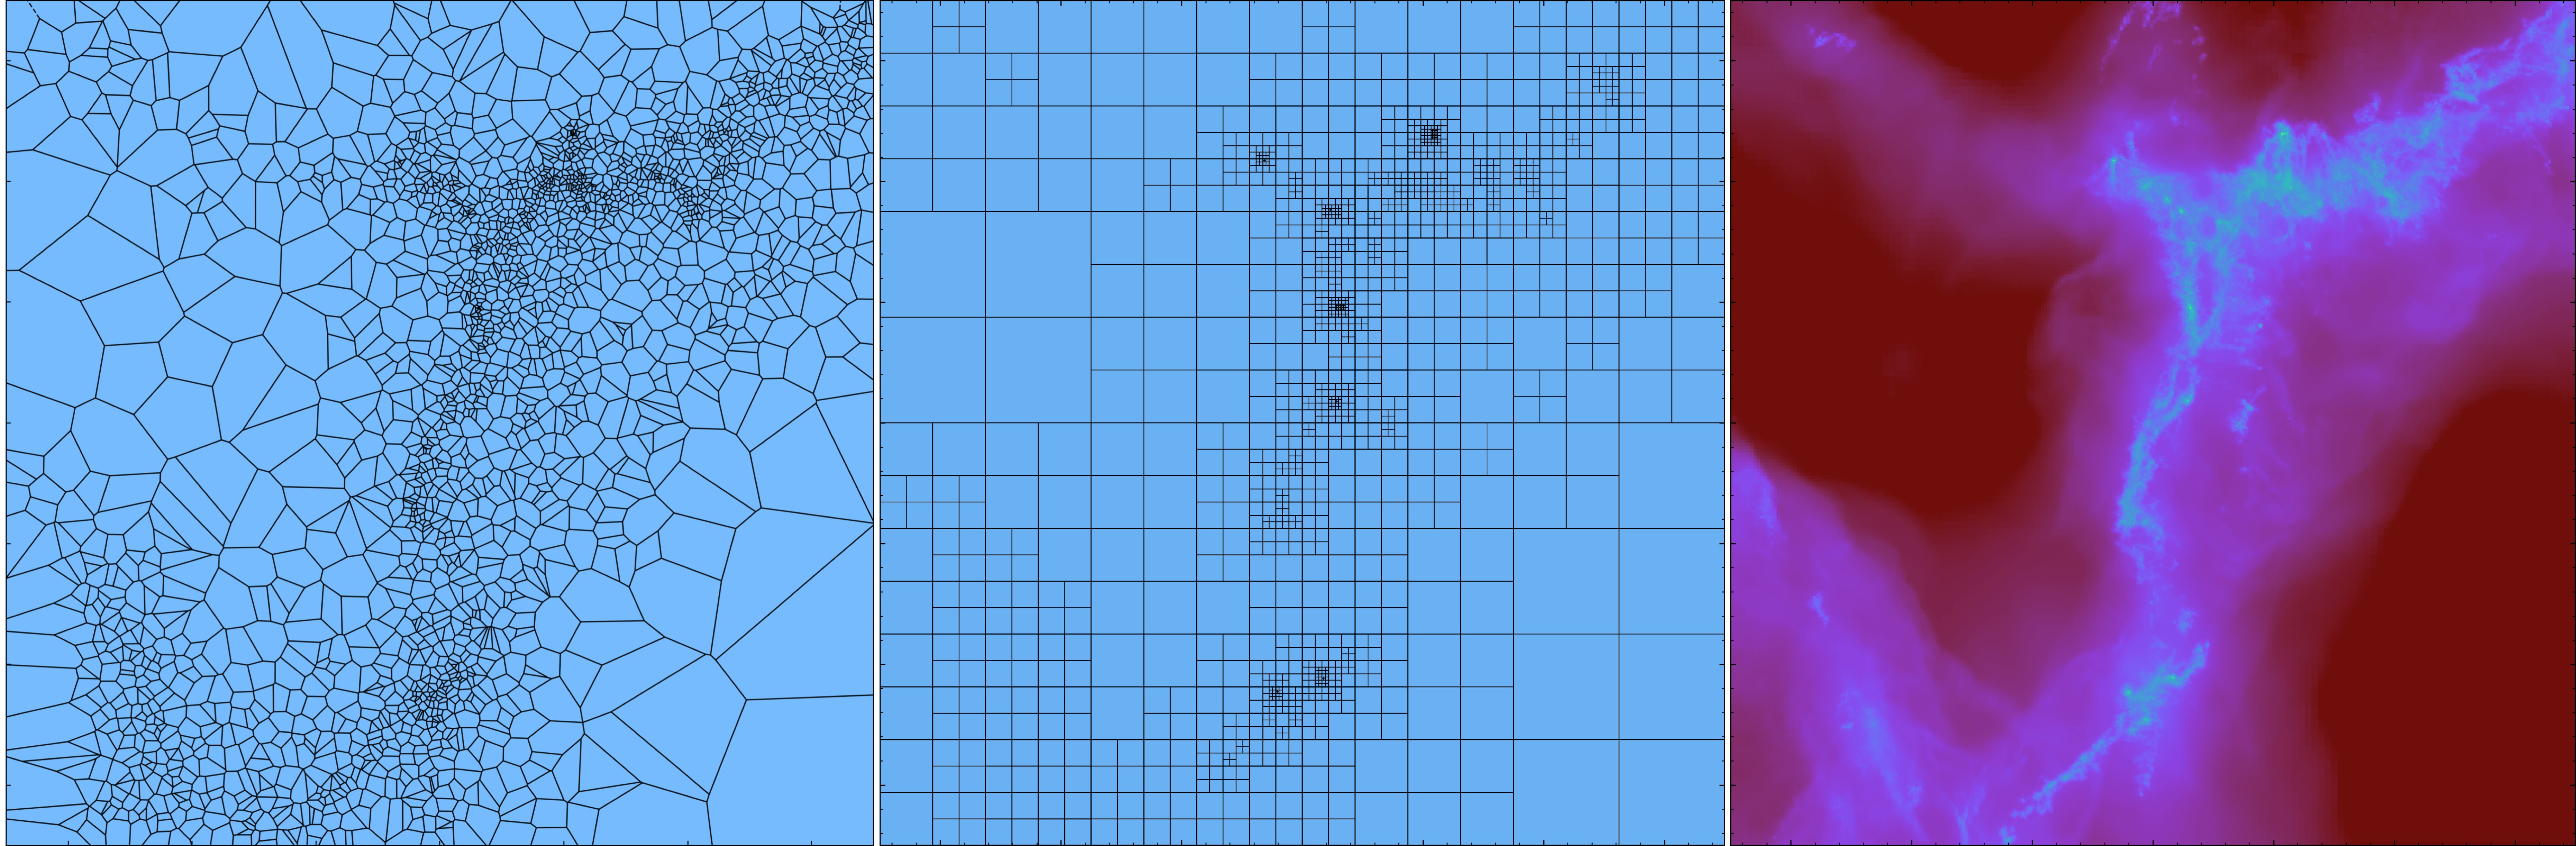
\includegraphics[width=0.99\linewidth]{3panel-building.png}
    \caption{Left: Voronoi mesh generated with the scipy.voronoi library from every 4096th data point of \arepo~source data (for visualization purposes). Middle:  Empty \flash~AMR grid generated from all \arepo~data with AMR blocks annotated and level 12 maximum refinement. Right: Populated \flash~AMR grid after \voramr~interpolation showing projected gas density; initial conditions of a Torch simulation.}
    \label{fig:building}
\end{figure*}

During refinement, each \flash~block is flagged to refine or de-refine until the contained-particle criterion is satisfied. The blocks of the AMR grid must also adhere to the restriction that neighboring blocks differ by no more than a single refinement level. This results in some regions of the computational domain being forced to over-refine such that they over-sample low density Voronoi cells. This method also does not guarantee that high-refinement Voronoi regions are interpolated into single \flash~grid cells, as a single cell may contain multiple Voronoi regions if the particles in a block are concentrated. This does lead to some data loss. We discuss the extent of this interpolation error in Section~\ref{sec:p2-proof}.

If the source data is not centered at (0,0,0), \voramr~detects the dimensions of the computational domain of the source data and performs a coordinate shift so that the data is centered at the origin. A similar centering is applied to the gas velocity data: the center of mass velocity of all gas in the domain is calculated and subtracted from the velocity field. This is a critical step, as the source data can still include bulk gas velocities representing the orbit of gas around the galaxy, which we do not model post-interpolation. \voramr~also accounts for unit changes between \arepo, which uses cosmological units, and \flash, which uses cgs units.

Figure \ref{fig:building} is an illustrative example of the stages of the \voramr~pipeline. Data is first extracted from the source file, in this case an \arepo~simulation of a collapsing GMC complex. Then, the structure of the source mesh is used to construct a \flash~grid that mimics the resolution of the source mesh by considering each mesh-generating particle as an object on which to refine. The empty grid is populated with source data with the nearest-neighbor interpolation scheme, and finally the grid is output as a \flash~checkpoint file. 

The checkpoint file produced by \voramr~can be read by other Torch versions to include physics or data-tracking not native to the original source data, such as binary star formation \citep{cournoyer-cloutier_implementing_2021,cournoyer-cloutier_early_2023}, controlled massive star formation \citep{lewis_early-forming_2023}, or protoplanetary disks \citep{wilhelm_modeling_2023,wilhelm_radiation_2023}.

\subsection{Source Data}
\begin{figure*}[!htb]    \includegraphics[width=\textwidth]{stacked_h_full.png}
    \caption{Left: the full \arepo~galaxy simulation from which the source data in this work is sampled. This galaxy is the SFE10 model detailed in \citet{li_effects_2020} Right: the zoom-in region used as source data for this work.}
    \label{fig:galaxy}
\end{figure*}

To illustrate the application of \voramr~to scientific data, we use a GMC complex extracted from a galaxy-scale star formation simulation computed using the \arepo~code and the SMUGGLE feedback module \citep{li_effects_2020}. GMCs of interest were chosen due to their future high rate of star formation. High resolution zoom-ins of these GMCs were then run in AREPO (see right panel in Figure \ref{fig:galaxy}.)
The complex detailed in this work is taken $\sim8$~kpc from the galaxy center. The zoom-in domain is $\sim1$~kpc per side. The total gas mass within the domain is $1.81\times10^7$~M$_{\odot}$. At the time we transfer data, 1\% of this gas has a temperature $<100$~K which is the regime that is most likely to be forming stars once evolved in Torch.

\subsection{Other Features}

%%% BACKGROUND GRAVITY
\subsubsection{Background Potential}
Often, astrophysical simulations include gravitational potentials from background influences such as dark matter. A consistent transfer of data between numerical frameworks must include such background potentials. The background-accel module in \voramr~allows for the calculation of the functional form of a static background gravitational acceleration. 

In the case of the \arepo~snapshots showcased here, there are softened massive particles that represent different components of the galactic gravitational potential. The particles represent a significant fraction of the mass present in the simulation snapshots, and so must be modeled to preserve the self-consistent nature of the initial conditions. Ideally, the particles would be included in the Torch framework as non-accreting, free moving, softened particles. However, some N-body codes that we wish to use through \amuse\ are not designed
to manage multiple particle types of differing softening lengths, so direct inclusion of background potential particles would require further code development.
Instead, we pass the background particles to a BHTree gravity solver \citep{barnes_hierarchical_1986} in \amuse~and sample the gravitational acceleration across the domain. We then pass that data through a median filter to smooth the influence of clumped background potential particles. We fit a one-dimensional, third-order polynomial that we use as the analytical solution to the background field in the vertical direction. The field can then be included into the Torch framework by calculating and adding the position-dependent background acceleration terms to the gravitational acceleration data array that \flash~produces with its gravity solver. The field remains constant throughout the simulation.

\subsubsection{Custom Zoom-In}

\begin{figure*}[!htb]
    \centering
    \includegraphics[width=0.99\linewidth
    ]{stacked_h_zoom_guidelines.png}
    \caption{Demonstration of \voramr's zoom-in capability. Any user-defined cubic region within the full computational domain (left) can be zoomed in to and evolved as a normal Torch simulation. Here, two zoom-in regions are shown, a 300\% zoom (center), and a 700\% zoom (right). All panels show projected gas density and have a maximum refinement level of 5, corresponding to a resolution of 5.6 pc, 1.87 pc, and 0.80 pc from left to right. Both zoom-ins are centered at the same point within the original computational domain to show the effect of enhanced detail while maintaining the same refinement level and criteria.}
    \label{fig:zoomin}
\end{figure*}
\voramr~can zoom in on user-specified regions of the given input data, as seen in Figure \ref{fig:zoomin}. This allows for higher refinement for regions of interest, as well as reduced computation time for the initialization of the grid. In this sense, \voramr~allows for a continuation of the GMC identification and zoom-in described by \citet{li_effects_2020}. To reduce the computational requirements, we mask out all input data that is not contained within the zoomed computational domain. The velocities of the interpolated gas are shifted to be relative to the gas center-of-mass velocity of the zoomed-in region. This helps ensure that the zoomed-in gas does not quickly exit the computational domain. One consideration, however, is that once a zoom-in is complete, gas data outside of the subregion is discarded and does not gravitationally affect and cannot enter the zoomed-in domain.

Zoom-ins must also properly account for the shift in background potential at the zoom-in location. We accomplish this by shifting the analytical background potential by the zoom-in center offset in z.

\subsubsection{Localized Refinement}
\begin{figure}[!htb]
    \includegraphics[width=\columnwidth]{roi-comparison-cropped.png}
    \caption{Comparison between AMR structure using full input data set (left) and localized refinement parameter (right). Local refinement is centered at the same point as the zoom-in regions in Figure~\ref{fig:zoomin}. The \flash~grid blocks are shown to demonstrate the reduction in total blocks necessary for a localized refinement.}
    \label{fig:localref}
\end{figure}

An alternative to using \voramr~to zoom in on regions of source data is to initially refine on user-specified regions of the given input data while forcing the rest of the domain to remain derefined. This solves two problems with zoom-in regions: (1) the resulting Torch evolution is cut off from the dynamical influence of the rest of the original source domain and does not experience tidal effects of gas structures from beyond the zoom-in region. (2)  surrounding gas can no longer flow into the zoomed-in region, which after a fraction of a crossing time becomes problematic. 


The user-specified refinement capability of \voramr~can use all the capabilities of the PARAMESH AMR library \citep{macneice_PARAMESH_2000} that forms the basis of the AMR in \flash. Focused refinement results in a significantly decreased computation time for initial grid construction and so is also an ideal method for visualizing subregions of an input domain. Figure \ref{fig:localref} shows two grids built using the same Voronoi source data, one allowing for refinement throughout the entire AMR domain, the other restricting refinement within a spherical region with a diameter of 150 pc. 

The localized refinement is accomplished by only passing \flash~the Voronoi source data within the refinement region. This way, the grid-building routines of \voramr~have no source data to refine on outside of the user defined region, restricting the refined portions of the domain. But, the \texttt{kdtree} from which data is interpolated is still built to contain source data from the entire domain. Therefore, \voramr~is still able to interpolate data across the entire domain regardless of whether the \flash~blocks lie within or outside the refinement region. Blocks outside the region of localized refinement will attempt to derefine to the minimum allowed refinement level. Note that PARAMESH requires there to be a maximum refinement level difference of 1 between neighboring blocks and so blocks immediately outside of the localized refinement region will be in some intermediate refined state. 

Maintaining a localized refinement region during a Torch run requires setting the grid refinement criteria of \flash~to override the other checks outside the local region that determine the refinement status of the blocks and whether to update that status. At the time of this writing, that override has not been implemented, so \voramr~can only initialize  regions of localized refinement. 

\section{Performance and Proof of Concept}\label{sec:p2-proof}

The interpolation of the source data into the \flash~grid  naturally results in errors. For example, if a single \flash~cell bounds a region occupied by multiple source data points, only the data closest to the \flash~cell center is brought onto the grid. In such an under-sampling case, caused either by tightly clumped source data or an insufficient maximum grid refinement level, some source data is lost. In general, under-sampling is not anticipated to be a large effect as any dropped data will typically be similar to the data that is interpolated onto the \flash~grid. Indeed, in using the same source data discussed throughout this paper, we find that while there is some error after interpolation in total mass, kinetic energy, and internal energy, none rise above 5\%, as seen in Figure~\ref{fig:error-graph}. 

Intuitively, we would expect a lower error at higher levels of refinement, but that is not seen. We suspect that at low refinement level grid cells act as broad smoothing filters, smearing a single \arepo~mesh element across coarse \flash~cells despite each cell often containing many mesh elements. However, source data in a slightly different orientation, say, offset by a few percent, is more likely to cause the error of the coarse grids to fluctuate as data interpolated into the cells are more likely to vary. Therefore, while a coarse grid will tend to average out any interpolation error that occurs, it is more likely to see a range of errors at low grid refinement, from very low to very high. We see this behavior in Figure~\ref{fig:error-graph}, where the interpolation error fluctuates at lower grid refinement but becomes more stable at higher refinement, as the grid structure approaches a comparable organization to the source \arepo~mesh. %{\bf This still doesn't explain the asymptotic behavior at high refinement.}
The error does not improve monotonically as refinement increases, this is most likely the result of the AMR grid structure approaching the limit of the smallest \arepo~mesh element dimensions.


\begin{figure}[!htb]
% GitRepos/Torch-Repositories/Torch-Analysis/voramrDev/error-analysis.ipynb
    \includegraphics[width=\columnwidth]{interpolation-error (1).png}
    \caption{Error in total mass, kinetic energy, and internal energy after first order nearest neighbor interpolation of \arepo~mesh data onto an AMR \flash~grid at various levels of maximum refinement. Solid lines represent the error from \flash~grids that are allowed to adaptively refine across the entire domain. Dashed lines are errors from \flash~grids that only refine in a region of interest 75 pc in radius representing 4.12\% of the original domain volume as seen in Figure~\ref{fig:localref}.
    %{\bf MM: can the full domain results be extended out to level 12?}
    }
    \label{fig:error-graph}
\end{figure}

Our Torch simulation uses sink particles \citep{federrath_modeling_2010}, the high perfomance $N$-body code \texttt{PeTar} \citep{wang_petar_2020} in conjunction with the binary and close encounter solvers \texttt{multiples} \citep{portegies_zwart_astrophysical_2018} and \texttt{smalln} \citep{hut_building_1995,mcmillan_binary--single-star_1996}, and the stellar evolution code \texttt{SeBa} \citep{portegies_zwart_population_1996}. We confirm that Torch initial conditions produced by \voramr~are well behaved when evolved. We initialize and evolve several Torch grids where the gas is largely bound, so we expect that it will readily form stars as it did in the original source simulation. Indeed, in these proof-of-concept simulations, sinks readily form,  gas continues to collapse, star particles are placed, and stellar feedback from ionizing radiation and winds behaves nominally. 

In comparing the evolved Torch simulation to the original \arepo~data, we find similarly located star forming regions after 3.2 Myr (Figure \ref{fig:runs}). Since \arepo~and Torch have entirely different methods for placing stars and introducing stellar feedback, we do not expect the two computational domains to look identical despite evolving from the same source data for the same amount of time. In addition, the preliminary Torch run shown here has a maximum refinement level of 5 with a resolution of 5.6 pc per cell side at the highest level of refinement. The \arepo~mesh has a minimum adaptive gas softening length of $\sim 1.7\times10^{-3}$~pc. The Torch run forms more compact clusters and 2.3 times as much stellar mass, $1.81\times10^5$~M$_\odot$ as compared to $7.87\times10^4$~M$_\odot$ in the \arepo~run. We reserve further investigation into these runs for following publications.

\begin{figure}[!htb]
\includegraphics[width=0.70\columnwidth]{star_formation_proof_labels.png}
    \caption{Gas column density at 3.22 Myr beyond the transfer time of {\em (top)} the source \arepo~simulation and {\em (bottom)} the Torch simulation. The black points are projected star particles that have formed from the gas.}
    \label{fig:runs}
\end{figure}

\section{Discussion}\label{sec:p2-discussion}
\subsection{Impact}
The translation of data from a Voronoi mesh onto an AMR grid provides an avenue for increased collaboration between researchers. Simulation frameworks grow robust and complex over time, leading to the tendency for researchers to become deeply entwined with unique but isolated software. This can lead to difficulties in translating computational advances made in one software framework to other frameworks. \voramr~enables researchers to collaborate with each other to maximize the reach and spread of their data and computational techniques. 

As a specific example of such collaboration, we show in this work how \voramr~becomes a critical linkage in the star cluster simulation pipeline, allowing researchers to initialize star cluster simulations using gas initial conditions from galactic-scale simulations. The star formation process is influenced by physics from an enormous range of length scales: galactic potential and outflows, down to the dynamics and feedback from individual stars. The range of length scales makes it prohibitively expensive for any one simulation to include all physical processes without significant approximations. For example, a simulation of an entire galaxy may include single particles that represent thousands or tens of thousands of stars or a simulation of a single GMC may include a background galactic potential without actually simulating the galactic dynamics. Researchers may also use idealized initial conditions for the gas cloud such as stirred boxes, turbulent spheres, or colliding cylinders. \voramr~enables star formation simulation frameworks like Torch to have access to realistic GMC initial conditions from galactic simulations. \voramr~provides an alternative to idealized initial conditions in Torch simulations.

\voramr~also provides a novel way to visualize Voronoi mesh-based hydrodynamical data. Voronoi meshes are notoriously difficult to produce visualizations from and researchers have often relied on sub-optimal approximations. A common method is to treat each Voronoi mesh cell as a particle and visualize the data using an SPH averaging kernel. This is not ideal as it smooths across the original Voronoi mesh data. Otherwise, researchers have transferred the Voronoi mesh data onto a uniform grid at the highest resolution of the model, which becomes infeasible for simulations with large dynamic ranges.  The advantage of the AMR grid is that it represents the same information at much lower cost in memory. Robust tools like \texttt{yt} \citep{turk_yt_2011} are built for efficiently visualizing large AMR grids. By interpolating onto an AMR grid \voramr~provides a form of mesh visualization without relying on the use of SPH kernel averaging. 

As it stands, \voramr~interpolates data from \arepo~simulations into the Torch framework, but in principle can be expanded to allow data from \emph{any} simulation suite to be translated into the Torch framework, including data from other Voronoi mesh codes, SPH representations, or even other AMR codes. 

\subsection{Limitations}
The interpolation of data from an \arepo~mesh into a \flash~grid results in a persistent error in the grid field values which is likely present even if \voramr~permits the grid refinement routine to refine until each block has an average of a single source mesh point per cell.
%mm 
%   {MM: this remains to be demonstrated}
Some error is of course expected, as a block-based AMR grid will never be able to exactly match the distribution of an unstructured mesh. We determine that the interpolation error reaches a few percent and remains consistent with increasing \flash~grid refinement, but further error testing is required for the highest refinement levels. Further development to implement higher order interpolation schemes should improve the interpolation error.

As it stands, \voramr~is closely tied to source data from \arepo~simulations and so can not yet be applied to a diverse set of input data structures. Because of the modular nature of \voramr~and Torch, future data structures such as other AMR grids as targets or SPH simulations as sources can be accommodated.

\voramr~detects and operates on \arepo~gas mesh-generating particles. \voramr~does not automatically handle other types of \arepo~ particles like star or wind particles. We have analytically derived an appropriate average background galactic potential based on the corresponding \arepo~particle set. We have not attempted to convert \arepo~star particles into Torch star particles. Therefore, the presence of \arepo~star particles represents a fraction of source domain total mass that is not interpolated onto the \flash~grid via \voramr. Neglecting such particles in the SMUGGLE model that we use results in only a fraction of a percent to a few percent of additional error in the total mass. 

\voramr~operates in serial, requiring a single processor to build the entire \flash~grid, which can take days for the production level models that we use. Future versions of \voramr~will parallelize the \flash~operations, users can still expect the grid building to take several hours for a sufficiently refined source data set (with millions or more mesh points corresponding to thousands of blocks). However, this operation only needs to be performed once at the start of a simulation. After interpolation, the simulation no longer requires \voramr~and takes full advantage of the parallelism in \flash.

The addition of persistent localized refinement to the Torch framework is still in development. Currently, the local refinement capability of \voramr~is useful for rapid production of AMR grids with regions of interest highly resolved. But once such a grid is evolved with Torch, the PARAMESH refinement criteria take over as normal and refine any blocks throughout the entire domain that satisfy the refinement criteria. A persistent localized refinement will allow for Torch runs with maximum levels of refinement which match the \arepo~mesh refinement without the computational cost of establishing that refinement across the whole AMR domain. Without persistent localized refinement, Torch runs using \voramr~interpolation will still be able to be processed but with a higher computational cost.

\section{Summary}
In this work we describe the use of the \amuse~framework to create a pipeline connecting the output Voronoi mesh data from \arepo~to input AMR grid data in \flash~to allow further evolution with the Torch star simulation framework. 

By using the \arepo~Voronoi mesh-generating particles to drive refinement, we use native \flash~routines to construct an empty adaptively refined grid.  We refine until there is an average of one mesh-generating particle per cell within each \flash~block (though we note that this still does not guarantee that every particle is in a separate cell). Simultaneously, we construct a $k$-dimensional lookup tree where each leaf node consists of the Cartesian coordinates of the \arepo~mesh-generating particle and the gas field values of density, internal energy, gravitational potential and three-dimensional velocity. We then use a first-order nearest neighbor interpolation scheme, taking advantage of the increased lookup speed of the k-d tree, to query and fill each \flash~cell with gas field values from the nearest \arepo~particle.

%mm [I hope we can rewrite this para]
We find that our interpolation scheme results in an error in global conserved quantities of total mass and energy of a few percent. Further indicating successful interpolation, gas within post-interpolation Torch runs continues to collapse to form multiple star clusters in filamentary structures over several megayears with no indications of numerical instability.

We describe several capabilities of the \voramr~data pipeline that work to provide a diversified range of uses in astrophysical simulation. Sub-regions of source data can be selected for interpolation onto the Torch-\flash~grid allowing for zoom-ins to regions of interest. We also provide a framework and proof of concept for future development in a localized refinement module to only permit sub-regions of the \flash~grid to undergo refinement. Lastly, we implement a background gravitational module so that additional gravitational influences from source data such as dark matter can be represented in the Torch simulation.

We note that the \voramr~data interpolation pipeline can be used for any source data so long as it can be represented as particles, though more robust interpolation methods would be needed for consideration of representations like SPH kernels.

We hope this work inspires similar efforts to build bridges between hydrodynamical simulation frameworks in promoting an open, interconnected scientific effort.

\section*{Data Availability}
The data from the simulations and figures within this article will be shared on reasonable request to the corresponding author. With the publication of this work, we make the \voramr~data interpolation pipeline public as part of the Torch distribution\footnote{\url{https://bitbucket.org/torch-sf/torch/src/vorch/}}.

\section{Acknowledgements}
This work was supported by NSF grants AST18-15461, AST-23-07950, and NSF ACCESS grant PHY220160. CCC is supported by a Canada Graduate Scholarship -- Doctoral from the Natural Sciences and Engineering Research Council of Canada (NSERC). We acknowledge John Zuhone for his consistent and timely assistance with \texttt{yt} visualizations and processing.

\emph{Facilities:} Snellius; SURF - Dutch National Supercomputing Center, Stampede2; Texas Advanced Computing Center

\emph{Software:} Torch \citep{wall_collisional_2019,wall_modeling_2020}, \amuse~\citep{portegies_zwart_multiphysics_2009,portegies_zwart_multi-physics_2013,pelupessy_astrophysical_2013,portegies_zwart_astrophysical_2018}, \flash~\citep{fryxell_flash_2000}, \texttt{yt} \citep{turk_yt_2011}, numpy \citep{oliphant_python_2007}, scikit-learn \citep{pedregosa_f_scikit-learn_2011}, matplotlib \citep{hunter_matplotlib_2007}, HDF5 \citep{koranne_hierarchical_2011}.


\chapter{Preliminary Results With VorAMR}\label{chp:Paper3}
\section{Regions of Interest}

\begin{figure*}
    \includegraphics[width=\linewidth]{roi-full-grid.png}\\
	\centering
    \caption{Top Left: the entire computational domain of the source \arepo~data. Panels A, B, and C are Torch snapshots from simulations with initial conditions interpolated from the corresponding cubic regions noted in the first panel. All plots are of gas density projection, the top two panels and bottom two panels share separate color bars as seen on the far right to allow the range of features to be visible in each spatial domain.}
    \label{fig:roi_grid_plot}

\end{figure*}
In Chapter \ref{chp:Paper2} we noted the custom zoom-in technique of VorAMR in which user-specified regions of source data are isolated from the rest of the source domain and magnified so that they may be evolved using Torch at higher resolution. As a proof of concept, we use VorAMR and Torch to identify and evolve three regions of interest from the source data GMC complex (as described in Chapter \ref{chp:Paper2}). The computational domain of these three simulations, as shown panels A, B, and C in Figure \ref{fig:roi_grid_plot} span a large spatial range. Region A has a domain side length of 30 pc, Region B is 430 pc, and Region C is 230 pc. The source region is $\sim1500$ pc on a side. At the maximum level of refinement, the corresponding minimum cell side length is 0.05 pc, 1.6 pc, and 0.9 pc for regions A, B, and C. There is a wide range of enclosed gas mass as well. The enclosed gas mass of Regions A, B, and C are $3.95\times10^4$~M$_\odot$, $1.34\times10^6$~M$_\odot$, and $2.92\times10^6$~M$_\odot$ respectively. The Regions are each evolved to allow for star forming regions to be identified. Computational requirements result in the Regions of higher zoom to take shorter time steps and so do not evolve as far in time. Region A is evolved for only 300 kyr, Region B for 3.2 Myr, and Region C for 1.9 Myr.

VorAMR allows for extraction of initial conditions from a single source data snapshot that span a spatial and total mass range of two orders of magnitude. These extracted initial conditions can vary greatly in morphology as well. Regions B and C highlight filament-like gas structures with star formation occurring along them while Region A is much closer to a spherical GMC like in Chapter \ref{chp:Paper1} but with a much more intricate initial state with a significant rotational component.

We strongly note that the panels in Figure \ref{fig:roi_grid_plot} are preliminary results and due to interpolation errors, which have since been corrected, are not intended to be published and are instead only visualizations of the capabilities and functionality of VorAMR.

\section{Comparison With AREPO}
\voramr~opens the door to a powerful mode of comparison between numerical frameworks. As described in Chapter \ref{chp:Paper2}, \voramr~uses a snapshot of data from an already computed \arepo~simulation and creates a set of initial conditions which can then be evolved by Torch. In this sense, \voramr~is a framework for direct side-by-side comparisons of \arepo~and Torch evolving from identical initial conditions.

As a proof of concept for such a comparison, we use \voramr~to convert an \arepo~simulation snapshot from the same simulation discussed in Chapter \ref{chp:Paper2} but from an early time step to allow both simulations to evolve independently for as long as possible. By using a snapshot from earlier in the \arepo~simulation we construct a \flash~grid from a much more coarse Voronoi mesh than in Chapter \ref{chp:Paper2}. As a consequence, \voramr~only constructs an AMR grid with a maximum refinement level of 4 (a minimum cell size of $11.2$~pc) to satisfy the interpolation criteria. We then evolve three separate Torch simulation from these initial conditions and permit each to achieve one higher level of refinement than the previous: a maximum level of 4, 5, and 6 (from here on referred to as lvl4, lvl5, and lvl6). After evolving the Torch simulations, we compare the rate of star formation to two \arepo~simulations, both of which have identical initial conditions but varying levels of stellar feedback. \arepo~simulation Aw0 has no stellar feedback, and Aw4 has ionizing radiationan and stellar wind feedback. We also include the data from the Torch run shown in Chapter \ref{chp:Paper2} which we refer to here as T2 and which was extracted by \voramr~2~Myr after the snapshot used for lvl4, lvl5, and lvl6.

\begin{figure}
    \centering
    \includegraphics[width=\linewidth]{sfr_arepo_comparison.png}
    \caption{Total mass of stellar material within the computational domains of a series of Torch and \arepo~simulations. Some data tracks do not begin from 0 (blue and green tracks) M$_\odot$ if the first appearance of star particles in the domain was a large burst of star formation.}
    \label{fig:sfr_comparison}
\end{figure}

In this preliminary investigation we find reasonable agreement between the Torch and \arepo~series of runs. Note the similarity in stellar mass growth between Tlvl5 and T2, both of which have a identical maximum refinements but are merely initiated from different \arepo~snapshots of the same GMC complex. We note that this mode of investigation has several caveats. Most notably, the stellar mass data from the Torch simulations track only new star formation and so this cumulative stellar mass can only increase in time as more stars form. We do not track star particles leaving the domain in the Torch runs nor do we track the injection of wind mass back into the domain as gas. In the \arepo~simulations, star particles from earlier stages of the simulation are actively entering and leaving the computational domain while stars are also forming. At this time we do not have a method for isolating these two components. As a result, the total stellar material in the \arepo~domains can trend downwards if more stars leave the domain than form within it. This method also does not track stellar wind mass that is injected back into the computational domain. However, the two \arepo~simulations behave as expected, with the run with no stellar feedback forming more stellar material than run Aw4. With these caveats in mind, we only intend to note the general similarities and order of magnitude adherence between the Torch and \arepo~simulations.

Naturally we expect the Torch and \arepo~simulations to diverge. Beyond the entirely different numerical hydrodynamical methods at play, the implementations of physics like radiation and stellar winds are also different. In addition, the mesh in the \arepo~simulation that we use in this comparison is able to achieve a significantly higher level of refinement than the Torch AMR grid. By the end of the simulation, the \arepo~mesh has a minimum adaptive gas softening length of $\sim 1.7\times10^{-3}$~pc and the Torch simulations have minimum cell side lengths of $11.2$~pc, $5.6$~pc, and $2.8$~pc. A Torch simulation with equivalent maximum resolution to the \arepo~simulation is possible but will require more computation time.

\chapter{Conclusions and Future Work}\label{chp:future}
\section{Conclusions}
In this work we use the numerical magnetohydrodynamics and N-body integrator code Torch to study aspects of star cluster formation, we also detail the development of a novel code which allows for simulation data from other numerical frameworks to be interpolated onto the FLASH AMR grid to be used as initial conditions in Torch simulations. 

In Chapter \ref{chp:Paper1} we designed a parameter study using the Torch simulation framework to investigate the effects of early-forming massive stars. We initialized a set of simulations of initially identical $10^4$~M$_\odot$ collapsing turbulent GMCs, and preemptively forcing either a 50, 70 or 100 M$_\odot$ star to form as early as possible. As a point of comparison, we also initialize a fiducial run in which from the same initial turbulent GMC, star formation occurs without user influence. We found distinct effects in the star cluster formation process due to the presence of an early-forming massive star. In the simulations containing an early-forming massive star, the gas of the natal giant molecular cloud becomes globally unbound $\sim$2 million years before the fiducial run, representing a significant impact on the star forming environment. This impact is further confirmed by our observation that the global star formation efficiency was reduced by a factor of three and the star formation efficiency per free-fall time was reduced by a factor of seven when compared to the fiducial run. Lastly, we found that early-forming massive stars both promote the formation of isolated stellar subclusters and hinders subcluster assembly into a single massive cluster. Early-forming massive stars reduce the ability for stars star clusters to form efficiently by both hindering the formation of individual stars and by halting the assembly of isolated subclusters.

In Chapter \ref{chp:Paper2} we announce VorAMR, a novel numerical tool which uses AREPO output data to construct a FLASH AMR grid onto which the AREPO hydrodynamical data is interpolated. VorAMR uses native FLASH routines to generate an empty AMR grid which refines in accordance to a distribution of Voronoi mesh generating particles. Then, a custom interpolation algorithm passes AREPO mesh data to the AMR grid via the AMUSE interface. VorAMR then produces a FLASH checkpoint file from which Torch simulations can be initiated. We note that the interpolation scheme results in an error of a few percent in global values total mass and total internal and kinetic energy. To our knowledge at the time of this thesis submission, VorAMR is first of its kind. VorAMR represents the bedrock of a revolution in numerical star formation simulations. We show that VorAMR can be successfully used to initialize Torch simulations with GMCs that formed in a galactic environment computed in AREPO. As a result, VorAMR essentially eliminates the need to use idealized GMC initial conditions such as turbulent spheres or colliding cylinders in Torch simulations. We note that the structure and logic of VorAMR can be adapted to interpolate data from any hydrodynamical data representation into a functioning Torch simulation such as SPH or other AMR frameworks.

In Chapter \ref{chp:Paper3} we discuss two preliminary investigations into a series of Torch star-cluster simulations using \voramr~interpolation. We confirm the versatility and ease-of-use of the custom zoom-in feature of \voramr~, detailing how subregions of an input \arepo~simulation snapshot can be extracted and evolved in Torch with no numerical abnormalities. We show that \voramr~can interpolate subregions of the original source data that span a significant spatial, mass, and resolution range. This capability allows researchers using Torch to evolve entire GMC complexes, individual GMCs, or subregions of single GMCs while taking advantage of the star formation and stellar feedback routines in Torch. We also detail a parameter study in which we track the stellar material within the computational domain of a series of Torch and \arepo simulations over sever megayears. This set of simulations are all initialized from the same \arepo~initial conditions, with the Torch simulations having passed through the \voramr~pipeline. The four Torch simulations have varying levels of refinement in order to quantify the effect of grid refinement on star cluster formation and evolution. The two \arepo~simulations have either none stellar feedback or ionization and stellar winds present. We find that the Torch and \arepo~simulations track fairly well with one another, noting that differences are expected since the Torch simulations presented are under-refined compared to the \arepo~simulations. We also note that as this is a preliminary study, the Torch simulations track only new star formation that occurs in their computational domain while the \arepo~simulations also track the entering and exiting of other star particles that formed prior to the simulation starting point, hence the \arepo~total stellar mass can increase and decrease while the Torch simulations can only increase. Within the set of future work set forth from this work, these initial investigation techniques will be refined.


\section{Future Work}
Torch is an extremely robust, extensive, and new numerical framework. As a result, many investigations and parameter studies are yet to be completed. In addition, Torch and its components are forever evolving, advancing, and being added to. The Torch research group consists of a dozen or so scientists in the US, the Netherlands, Germany, Canada, Mexico, and Kazakhstan. Much work to expand Torch and explore its capabilities is currently underway. Here we detail a few major points of future work that will naturally grow out of the work presented in this thesis.

\subsection{Further Parameter Studies in Torch}
One under-explored parameter space is the method by which star particles are placed in Torch. Torch forms star particles from sink particles based on the stellar mass list and how much gas the sink has accreted. Once the sink has accreted enough mass to form the next star in the list, the star particle is assigned a position derived from a 3D Gaussian distribution centered at the position of the parent sink. The assumption is that because sinks represent sub-grid (unresolved) gas dynamics, the gas will most likely continue collapsing to a centrally concentrated distribution, making stars more likely to form there. But, it is also reasonable to assume that since we cannot resolve the gas behavior inside of sinks, new stars should be assigned a position using a uniformly random 3D distribution within the sink. Altering the star placement procedures will have implications for early cluster evolution and whether a cluster is likely to be disrupted.

Other future additions to Torch include new stellar feedback mechanisms. So far, Torch includes feedback from massive stars. However, at the earliest stages of star cluster formation, when massive stars may not have formed yet, including feedback from low mass stars may be critical to building an accurate numerical model. Specifically, jets from low mass stars are thought to drive gas turbulence, injecting energy and momentum into their surroundings and reducing star formation efficiency \citep{bally_protostellar_2016}.

\subsection{VorAMR Extensions}
VorAMR is an incredibly powerful tool, and yet its logic and code organization (see Appendix \ref{app:voramrsource}) is relatively simple. Along with its purposeful modular design with respect to Torch, VorAMR can be easily extended within the Torch framework or adapted to be used in other AMR simulation frameworks. Possible extensions are numerous. Here we list several where development work has already begun.

One such improvement to VorAMR is the parallelization of the grid refinement step. The time to parse the source data and interpolate the data onto the refined FLASH grid is negligible compared to the time required to construct the refined FLASH grid. Constructing the grid is computationally intensive and is expected to take significant resources (though such as requirement is worthwhile since it only need be performed once per run). To make matters worse, the FLASH worker within a VorAMR execution currently operates using a single processor. FLASH is designed to operate in parallel with suggestions to compute $\sim100$ grid blocks per processor. VorAMR can have thousands of blocks on a single processor, potentially resulting in steep slowdowns as the processor is oversubscribed. Parellelization of VorAMR would require modeling the source data read-in steps to more closely mimic the initial conditions methods of a standard Torch run. 

VorAMR should also be expanded to allow other source and output data types to be used. As of this publishing, VorAMR can only read AREPO particle data and output FLASH grid data. The modular nature of VorAMR allows for the addition of alternate data parsing functions to be used in cases of differing source or output data organization, easily controllable by user parameters. The philosophy and logic of VorAMR can accept and interpolate data from any source so long as the data can be represented by particles. VorAMR can, in principle, create Torch initial conditions from \emph{any} SPH, moving mesh, or AMR code. The logic and philosophy of VorAMR should also be integrated into other computational frameworks beyond Torch and FLASH. Conversations with researchers who work with the AMR grid code RAMSES \citep{teyssier_cosmological_2002} indicates that VorAMR grid construction and interpolation can be fully integrated with relative ease. In a related effort, VorAMR should be incorporated into the AMUSE framework distribution to increase its accessibility to other researchers.

The analysis of VorAMR interpolated Torch runs as described in Chapter \ref{chp:Paper2} should be extended. VorAMR presents an opportunity to perform direct comparisons between star cluster formation and evolution as it takes place across two or more numerical frameworks given the same complex initial conditions. Such a robust form of numerical comparison has not yet been performed in star cluster formation research. 


%Ideally, this localized refinement restriction would be made to be permanent over many simulation evolution steps. This way the dynamical influence of gas and stars of extensive regions to remains influential on a highly refined region of interest without requiring VorAMR to process the refinement of the entire computational domain. Though this method is still in development.


\end{thesis}

\bibliography{finalbib-no-doi} % Include references.bib BibTeX


\appendix
\chapter{VorAMR Details}
\section{VorAMR flash.par additions}
The \voramr~addition to the Torch framework is controlled through the \flash~parameter file \texttt{flash.par}. The relevant additions are listed here.
\begin{lstlisting}[language=bash]
# ================
# VorAMR extension
# ================
use_voramr = .true.
voramr_source = "snapshot_518_9.hdf5" # data from non-Torch simulation
voramr_input = "voramr_input.hdf5" # cleaned up FLASH readable source data

refine_on_particle_count = .true.
min_particles_per_blk    = 4096 # Assumes 16x16x16 blocks
max_particles_per_blk    = 4096
pt_maxPerProc            = 10000000 # Enough to fit all particles on one proc
#refine_var_2 = "dens"
refineonjeanslength = .true. #.false.

# Restrict initial refinement by only placing particles within radius
use_localRef = .true.
center_localRef = .true.
localRef_x = 0.0 
localRef_y = 4.628517e+20 # 150 pc 
localRef_z = 0.0 
localRef_r = 4.363807e+20 # 141.421 pc 

# Background Potential
sim_withStaticGrav = .true.
              # AREPO 518_9 \ # Hill et al 2012
sim_aParm1  = 1.31142525e-72  #4.39996789e-9  # [cm/s^2]     # 1.42E-3 [kpc/Myr^2]
sim_aParm2  = 1.35401904e-52  #5.51293615e-31 # [1/s^2]      # 5.49E-4 [1/Myr^2]
sim_aParm3  = -2.36078509e-30 #5.55421965e20  # [cm]         # 0.18E0  [kpc]
sim_aParm4  = 4.06112841e-11  #1.62715932e-53 # [1/(cm s^2)] #5 .0E-5  [1/kpc Myr^2]
\end{lstlisting}

\section{VorAMR Installation and Operation Steps}
This guide assumes that you have already followed and completed the Torch installation steps detailed in the Torch quickstart guide, found on the Torch public facing website\footnote{\url{https://torch-sf.bitbucket.io}}. 
\begin{itemize}
    \item [] 1. Change VorAMR flags to .true. in flash.par (use\_voramr, refine\_on\_particle\_count).
    \item [] 2. Change voramr\_source to input source file name (assumes file is in same directory as Torch run). voramr\_input should not be changed, VorAMR will always output a FLASH-readable HDF5 file with the name "voramr\_input.hdf5".
    \item [] 3. \{min,max\}\_particles\_per\_blk should remain 4096 unless more/less strict refinement criteria are desired.
    \item [] 4. pt\_maxPerProc should be changed such that 1 processor can handle all source data particles.\\

-- Steps 5 and 6 vary depending on your intentions to zoom, locally refine. --\\

Assuming no zoom in and no local refinement:
    \item [] 5. use\_localRef and center\_localRef turned to .false. (localRef\_\{x,y,z\} then have no effect)
    \item [] 6. Set \{x,y,z\}min and {x,y,z}max in flash.par to enclose entire source data particle set.\\

Assuming zoom in:
    \item [] 5. use\_localRef and center\_localRef turned to .true. (localRef\_\{x,y,z\} now define center of zoom region in reference to source data). Set localRef\_r to $\sqrt{2}\times$domain side length.
    \item [] 6. Set \{x,y,z\}min and \{x,y,z\}max in flash.par to zoom in dimensions making sure to match localRef\_r requirement.\\

Assuming local refinement:
    \item [] 5. use\_localRef turned to .true. and center\_localRef turned to .false. (localRef\_\{x,y,z\} now define center of refinement region in reference to source data).
    \item [] 6. Set \{x,y,z\}min and \{x,y,z\}max in flash.par to enclose entire source data particle set.\\

-- All runs perform the following steps --\\

    \item [] 7. If a background potential is desired, turn sim\_withStaticGrav to .true. and give polynomial coefficients in sim\_aParm\{1,2,3,4\}.
    \item [] 8. Set tmax and checkpointFileIntervalTime to 1.1 dtmin (this ensures a populated FLASH grid and checkpoint file is output before the run completes).
    \item [] 9. Set lrefine\_max to whatever max refinement you want. VorAMR may stop refinement early if refinement criteria are satisfied. lrefine\_min should stay at 2.
    \item [] 10. Run Torch simulation. Three checkpoint files will be produced with numeration 0000, 0001, 0002. 0000 is an empty grid, 0001 is output immediately after VorAMR refinement and interpolation, 0002 is output after 1 FLASH step.
    \item [] 11. Use checkpoints 0001 or 0002 as restart file in a standard Torch build.
\end{itemize}

\section{VorAMR Source Code}\label{app:voramrsource}
Additions to Torch framework:

\begin{lstlisting}[language=python]
from scipy.interpolate import NearestNDInterpolator
import h5py
import numpy as np
import pickle
from .datamodel import Particles
from .units import units
from datetime import datetime

def read_hdf5(file_path):
    """
    Opens an hdf5 data file and extracts the coordinates
    of the Voronoi cells (or other data structures)
    as well as the associated gas desnity, 
    internal energy, and velocity field values. 
    
    This function is written specifically to expect AREPO output
    data. Other data structures will need to have tailored calls
    to extract the data from the hdf5 file structure. Hopefully
    you'll only have to edit this file though!
    
    Arguments:
    file_path - input AREPO hdf5 file path

    Returns:
    coords    - list containing 3 1xN numpy arrays representing the 
                x, y, z coordinate sets for all Voronoi cells.
    field_set - 5xN numpy array where the columns are the separate
                field values of interest (density, internal energy,
                velx, vely, velz).
    """
    f = h5py.File(file_path,'r')
    coords_set = np.array(f["PartType0"]["Coordinates"])
    x = coords_set[:,0]
    y = coords_set[:,1]
    z = coords_set[:,2]
    coords = [x,y,z]

    # Extract field values from AREPO HDF5
    density_set = np.array(f["PartType0"]["Density"])
    intEner_set = np.array(f["PartType0"]["InternalEnergy"])
    mass_set = np.array(f["PartType0"]["Masses"])
    velocity_set = np.array(f["PartType0"]["Velocities"])
    # We need to separate velocity vector, need to interpolate each component
    velx = velocity_set[:,0]
    vely = velocity_set[:,1]
    velz = velocity_set[:,2]
    gpot = np.array(f["PartType0"]["Potential"]) 

    field_set = np.stack((density_set, intEner_set, velx, vely, velz, gpot), axis=-1)
    return coords, field_set

def build_kdtree(coords, field_set):
    """
    Builds KDtree object from N coordinates and m x N field values.
    Each leaf of the tree corresponds to a Voronoi cell center with m 
    field values associated with that cell.

    Arguments:
    coords    - coordinate set [x, y, z] where x,y,z are 1 x N numpy arrays.
    field_set - m x N array of field values.

    Returns:
    tree      - kdtree object with field value matrix on each leaf node.
    """
    # Create interpolator object (tree)
    tree = NearestNDInterpolator(list(zip(coords[0], coords[1], coords[2])), field_set)
    return tree


def pickle_tree(tree, file_out_name):
    """
    Pickles any object. Syntax tailored specifically for tree
    structures produced by the functions in voramr_kdtree.py.
    The pickled tree object can be accessed an interpolated from
    without having to re-generate the tree.

    Arguments:
    tree          - tree (or any other) object to be pickled.
    file_out_name - file name to be saved in current directory.
    """
    # Pickling tree
    file_w = open(file_out_name, 'wb')
    pickle.dump(tree, file_w)
    file_w.close()
    return

def unpickle_tree(file_in_name):
    """
    Unpickles an object and returns it.

    Arguments:
    file_in_name - name/path of pickle file.

    Returns:    
    tree_struct - unpickled tree (or any other object).
    """
    file_r = open(file_in_name, 'rb')
    tree_struct = pickle.load(file_r)
    file_r.close()
    return tree_struct


def interp_data(tree_struct, cell_coords):
    """
    Performs Nearest Neighbor interpolation between single cell
    3d coordinates and a KDtree and returns the values associated
    with the nearest tree leaf (Voronoi cell center).

    Arguments:
    tree_struct - KDtree structure.
    cell_coords - [x, y, z] coordinates of single cell.

    Returns:
    interp_data - field values of nearest neighbor between cell 
                  coordinates and a KDtree leaf.
    """
    interp_data = tree_struct(cell_coords[0], cell_coords[1], cell_coords[2])
    return interp_data


def extract_data(file_name, apply_consts=True):
    #pctocm, kmtocm, msuntog, scale0, scale1  = 1, 1, 1, 1, 1
    if (apply_consts):
        # AREPO uses different units than FLASH, these are the conversions.
        # https://www.illustris-project.org/data/docs/specifications/
        length, mass, velocity, hubble = 3.08567759e+21, 1.989e43, 1.0e5, 0.7
    f = h5py.File(file_name, 'r')
    ds = f['PartType0']
    c = ds['Coordinates'][:]*length*(1./hubble)
    d = ds['Density'][:]*mass*(hubble**2)*(1./length**3)
    m = ds['Masses'][:]*mass*(1./hubble)
    ie = ds['InternalEnergy'][:]*velocity**2
    v = ds['Velocities'][:]*velocity
    gpot = ds['Potential'][:]*velocity**2
    
    coords = np.array([c[:,0], c[:,1], c[:,2]]).T
    vels = np.array([v[:,0], v[:,1], v[:,2]]).T

    #Extract star dataset
    sds = f['PartType4']
    c = sds['Coordinates'][:]*length*(1./hubble)
    sm = sds['Masses'][:]*mass*(1./hubble)
    im = sds['GFM_InitialMass'][:]*mass*(1./hubble)
    v = sds['Velocities'][:]*velocity
    a = sds['GFM_StellarFormationTime'][:]
    smet = sds['GFM_Metallicity'][:]

    scoords = np.array([c[:,0], c[:,1], c[:,2]]).T
    svels = np.array([v[:,0], v[:,1], v[:,2]]).T
    f.close()
    return coords, vels, d, m, ie, gpot, scoords, svels, sm, im, a, smet

def rescale_coords_vels(coords, vels, masses, scoords, svels, use_com_coords=False):
    #pctocm, kmtocm, msuntog, scale0, scale1  = 1, 1, 1, 1, 1
    #u_coord = units.pc
    #u_vels = units.km/units.s
    #if (apply_consts):
        #pctocm, kmtocm, msuntog, scale0, scale1 = 3.08567759e+18, 1.0e5, 1.989e33, 0.7e3, 0.7e10
    u_coord = units.cm
    u_vels = units.cm/units.s
    # This is a pretty crude method for centering the domain at (0,0,0)cm but it works for now.
    x_cor = (coords[:,0].max()+coords[:,0].min())/2
    y_cor = (coords[:,1].max()+coords[:,1].min())/2
    z_cor = (coords[:,2].max()+coords[:,2].min())/2
    
    parts = Particles(len(vels[:,0]))
    parts.x, parts.y, parts.z = coords[:,0] | u_coord, coords[:,1] | u_coord, coords[:,2] | u_coord
    parts.vx, parts.vy, parts.vz = vels[:,0] | u_vels, vels[:,1] | u_vels, vels[:,2] | u_vels
    parts.mass = masses
    
    if (use_com_coords):
        # Set the center of mass as (0,0,0)cm
        com_coords = parts.center_of_mass().value_in(u_coord)
        x_cor, y_cor, z_coor = com_coords[0], com_coords[1], com_coords[2]

    # Scale velocities such that center of mass of system is (0,0,0)cm/s
    com_vels = parts.center_of_mass_velocity().value_in(u_vels)
    vx_cor = com_vels[0]
    vy_cor = com_vels[1]
    vz_cor = com_vels[2]

    coords_cor = coords - np.array([x_cor, y_cor, z_cor]).reshape(1,3)
    vels_cor = vels - np.array([vx_cor, vy_cor, vz_cor]).reshape(1,3)

    # Same for stars if we have them
    scoords_cor = scoords - np.array([x_cor, y_cor, z_cor]).reshape(1,3)
    svels_cor = svels - np.array([vx_cor, vy_cor, vz_cor]).reshape(1,3)
    return coords_cor, vels_cor, scoords_cor, svels_cor

def write_corrected_file(output_filename, coords, vels, dens, masses, ie, gpot,
                         scoords, svels, smass, sinitmass, sfmtime, smetal,
                         use_localRef=False, local_ref=[0.0,0.0,0.0], recenter_coords=False):
    # Write all gas data to file to be included in interpolation kdtree regardless if we
    # are refining on a region of interest. Include all field values.
    #f = h5py.File("kdtree-"+output_filename, 'w')
    f = h5py.File("interp-data.hdf5", 'w') 
    group = f.create_group('PartType0')
    coords_i = coords.copy()
    if (local_ref and recenter_coords):
        # Only want to limit what we write to interpolation file if we are rescaling coords,
        # since then we are presumably zooming in on ROI and do not need to interp
        # to full computational domain.
        locx, locy, locz, locr = local_ref[0], local_ref[1], local_ref[2], local_ref[3]
        diffr = np.sqrt((coords[:,0]-locx)**2 + (coords[:,1]-locy)**2 + (coords[:,2]-locz)**2)
        ind = np.where(diffr < locr)
        # Set particle coord array to be only those within ROI.
        coords_i = coords.copy()[ind]
        vels = vels[ind]
        masses = masses[ind]
        vprint("Shifting coordinates and velocities of interpolation file for recentered local refinement")
        # RESCALING SCOORDS AND SVELS FOR ROI NOT IMPLEMENTED YET - SCL 04/15/23
        coords_cor, vels_cor, scoords_cor, svels_cor = rescale_coords_vels(coords_i, vels, masses, scoords, svels, use_com_coords=False)
        coords_i = coords_cor
        vels = vels_cor
        dens = dens[ind]
        ie = ie[ind]
        gpot = gpot[ind]
    vprint("{} particles saved to interp-data.hdf5".format(len(coords)))
    dset = group.create_dataset('Coordinates', data=coords_i, dtype='d')
    dset = group.create_dataset('Velocities', data=vels, dtype='d')
    dset = group.create_dataset('Density', data=dens, dtype='d')
    dset = group.create_dataset('Masses', data=masses, dtype='d')
    dset = group.create_dataset('InternalEnergy', data=ie, dtype='d')
    dset = group.create_dataset('Potential', data=gpot, dtype='d')
    f.close()
    #vprint("Wrote all gas field values to", "kdtree-"+output_filename)
    vprint("Wrote all gas field values to", "interp-data.hdf5")
    
    
    if(use_localRef):
        vprint("DOING LOCALIZED REFINEMENT. Limiting gas particles written. Opening",output_filename)
        # open file to fill with region-of-interest gas only --> FLASH refinement
        # therefore only need coordinate data, commented out all other field values
        # to reduce file size.
        f = h5py.File(output_filename, 'w')
        group = f.create_group('PartType0')
        
        locx, locy, locz, locr = local_ref[0], local_ref[1], local_ref[2], local_ref[3]

        # New addition 04/18/23 extracting particles inside cube of side 2/sqrt(2)*locr centered at loc{x,y,z}
        # From https://stackoverflow.com/questions/42352622/
        vprint("Creating new mask for particles in bounding cube of side 2*locr/sqrt(2)")
        sqrt2 = np.sqrt(2)
        bound_x = np.logical_and(coords[:, 0] > locx-locr/sqrt2, coords[:, 0] < locx+locr/sqrt2)
        bound_y = np.logical_and(coords[:, 1] > locy-locr/sqrt2, coords[:, 1] < locy+locr/sqrt2)
        bound_z = np.logical_and(coords[:, 2] > locz-locr/sqrt2, coords[:, 2] < locz+locr/sqrt2)
        bb_filter = np.logical_and(np.logical_and(bound_x, bound_y), bound_z)
        coords = coords[bb_filter]

        if (recenter_coords):
            x_cor = (coords[:,0].max()+coords[:,0].min())/2
            y_cor = (coords[:,1].max()+coords[:,1].min())/2
            z_cor = (coords[:,2].max()+coords[:,2].min())/2
            coords = coords - np.array([x_cor, y_cor, z_cor]).reshape(1,3)
        dset = group.create_dataset('Coordinates', data=coords, dtype='d')
    else:
        vprint("USING ALL GAS PARTICLES, NO LOCAL REFINEMENT.")
        # open file to fill with ALL gas data --> FLASH refinement
        # also would only need coordinate data.
        f = h5py.File(output_filename, 'w')
        group = f.create_group('PartType0')
        vprint("coords shape: ", coords.shape)
        vprint("masses shape: ", masses.shape)
        dset = group.create_dataset('Coordinates', data=coords, dtype='d')

    vprint("Wrote FLASH refinement gas and stars to", output_filename)
    f.close()


def get_leaf_blocks(hydro, cellsPerBlock=16, numBlocks=None):
    """
    Acquires all FLASH blocks representing the computational domain.
    
    Arguments:
    hydro         - instance of  flash_worker.
    cellsPerBlock - number of cells in each direction of a FLASH block.
    numBlocks     - number of blocks in the computational domain. 
                This is passed in by the user, as long as numBlocks 
                is > the actual number of blocks in the domain, 
                this routine runs fine. 

    Returns:
    leaf_grids[:numblks] - list of active blocks. The slicing removes
                           any extra buffers that are present from
                           passing too many numBlocks.
    """
    vprint("Getting block data...")
    lim=cellsPerBlock
    lim3 = lim**3

    vprint("getting leaf_indices")
    all_grids=numBlocks # hard coded from torch_user.py. Can be set arbitratily large to
                        # accomodate any sized grid.
    [leaf_grids, block_array, num_leafs]= hydro.get_leaf_indices(list(range(all_grids)))
    numblks=num_leafs[0]
    
    leaf_grids = np.resize(leaf_grids,numblks*lim3)
    
    return leaf_grids[:numblks]

def interpolate_fields(hydro, leaf_grids, kdtree, cellsPerBlock=16):
    """
    This subroutine loops over each block in the computational domain
    and does three things. 
    1.) The x,y,z coordinates of all cells
    within the block are extracted and transformed into a 3D numpy
    meshgrid. 
    2.) The coordinate mesh is passed to the kdtree 
    interpolator and nearest neighbor interpolation is performed on
    each cell within the mesh resulting in a 4D NxNxNxM matrix where
    N is the dimensionality of the FLASH block and M is the number of
    field values interpolated. 
    3.) The inerpolated field values
    are unraveled one by one from the 4D matrix and flattened into an
    ordered 1D array and fed back into FLASH. FLASH is smart enough
    to fill the 3D block matrix from a 1D array.
    
    Arguments:
    hydro      - instance of  flash_worker.
    leaf_grids - list of active blockIDs.
    kdtree     - 3D tree object built previously from the input data, 
                 allows for nearest neighbor interpolation.
    """
    lim = cellsPerBlock
    a = np.empty(lim)
    a.fill(1)
    b = np.empty_like(a)
    b.fill(2)
    c = np.empty_like(a)
    c.fill(3)
    vprint("Getting {} block cell coords, interpolating, pass back to FLASH.".format(leaf_grids[-1]))
    for leaf in leaf_grids: # Cycle over BlkIDs
        # Get x, y, z coordinates of cells in BlkID==leaf
        x = np.array(hydro.get_1blk_cell_coords(a,leaf,lim).value_in(units.cm))
        y = np.array(hydro.get_1blk_cell_coords(b,leaf,lim).value_in(units.cm))
        z = np.array(hydro.get_1blk_cell_coords(c,leaf,lim).value_in(units.cm))

        # Mesh coordinates into single 3D matrix object
        coords_mesh = np.meshgrid(x,y,z,indexing='ij')
        
        # Pass coordinate mesh into kdtree interpolation, get field values for each coord point.
        interp = interp_data(kdtree, coords_mesh)
        
        # Using interpolated data. Flatten to 1D to feed to Fortran.
        rho = interp[:,:,:,0].flatten(order='F') | units.g/units.cm**3
        eint = interp[:,:,:,1].flatten(order='F') | (units.cm**2)/(units.s**2)
        vx = interp[:,:,:,2].flatten(order='F') | units.cm/units.s
        vy = interp[:,:,:,3].flatten(order='F')	| units.cm/units.s
        vz = interp[:,:,:,4].flatten(order='F') | units.cm/units.s
        gpot = interp[:,:,:,5].flatten(order='F') | (units.cm**2)/(units.s**2)
        
        dataSize = cellsPerBlock
        
        # Feed field data to FLASH.
        #Fortran can properly populate its NxNxN matrices when given a 1xN^3 matrix
        hydro.set_block_state(leaf, dataSize, rho, vx, vy, vz, eint, gpot)
        
    vprint("Done setting blocks. Total blocks: ", leaf)

def vprint(*args, **kwargs):
    vstr = (datetime.now().strftime("%m-%d-%Y %H:%M:%S.%f"))[:-3]
    print("[VorAMR {}] ".format(vstr), end='')
    return print(*args, **kwargs)


def run_torch(user_initial_conditions, user_parameters):
    """
    Run a Torch simulation.  This is called from a user script, which provides
    initial conditions and parameters for the desired problem set up.

    Arguments: requires two methods as input.

        user_initial_conditions(state, hydro) - method that alters "state", "hydro" objects to set initial conditions for simulation.

        user_parameters() - method that returns a dict of Torch configuration parameters

    Result: spawn the necessary FLASH, gravity, stellar evolution, etc. workers
    to run a Torch simulation.  Attempt to run the simulation to completion.
    """

    global USER
    USER = user_parameters()

    tprint("Num hydro workers: {:d}".format(USER['num_hy_workers']))
    tprint("Num grav workers: {:d}".format(USER['num_grav_workers']))
    tprint(" overwrite: {}".format(USER['overwrite']))

    if USER['npy_seed'] is not None:
        np.random.seed(USER['npy_seed'])
    if USER['with_voramr']:
        tprint("Initializing with VorAMR.")
        if USER['convert_file']:
            vprint("Converting  provided hdf5 file.")
            coords, vels, dens, mass, eint, gpot, scoords, svels, smass, sinitmass, sfmtime, smet = extract_data(USER['source_file'], apply_consts=True)
            coords_cor, vels_cor, scoords_cor, svels_cor = rescale_coords_vels(coords, vels, mass, scoords, svels, use_com_coords=False)
            write_corrected_file(USER['input_file'], coords_cor, vels_cor, dens, mass, eint, gpot, scoords_cor, svels_cor, smass, sinitmass, sfmtime, smet, USER['use_localRef'], USER['local_ref'], USER['center_local_ref'])
            coords, field_set = read_hdf5("interp-data.hdf5")
        else:
            vprint("Using unconverted source file.")
            coords, field_set = read_hdf5(USER['source_file'])

        vprint("Building field interpolator.")
        kdtree = build_kdtree(coords, field_set)
        if(USER['pickle_kdtree']):
            pickle_tree(kdtree, USER['pickle_file_name'])
            vprint('Pickled kdtree: {}'.format(USER['pickle_file_name']))
    # End VorAMR file init
    
    hydro, grav, mult, se = initialize_workers()

    # After hydro initialize, interpolate data onto grid if using VorAMR.
    if USER['with_voramr']:
        vprint("Interpolating external data to FLASH grid via VorAMR.")
        leaf_blocks = get_leaf_blocks(hydro, cellsPerBlock=USER['cellsPerBlock'], numBlocks=USER['numBlocks'])
        interpolate_fields(hydro, leaf_blocks, kdtree, cellsPerBlock=USER['cellsPerBlock'])
        vprint("Done interpolating. VorAMR complete.")

    state = TorchState(hydro, grav, mult)

    state.initial_io(overwrite=USER['overwrite'], refresh=USER['restart_with_new_rng'])
    
    if not state.restart:
        user_initial_conditions(state, hydro)
    elif state.restart and USER['restart_with_user_ics']:
        # massage the hydro particle structures so that particles from user ICs
        # look like they came from restart checkpoint file.
        hydro.set_starting_local_tag_numbers()
        user_initial_conditions(state, hydro)
        hydro.clear_new_tags()

    try:

        evolve(state, hydro, grav, mult, se)

    finally:
        pass
\end{lstlisting}

\noindent Additions to  interface:

\noindent\textbf{base\_grid\_interface.F90}
\begin{lstlisting}[language=fortran]
FUNCTION set_block_state(blockID, dataSize, rho, vx, vy, vz, eint, gpot)
  INTEGER :: blockID
  INTEGER :: dataSize
  DOUBLE PRECISION,dimension(dataSize,dataSize,dataSize) :: rho, vx, vy, vz, eint, gpot
  INTEGER :: set_block_state !beginCount, set_block_state
  INTEGER,dimension(3) :: startPos, dataDims
  startPos = [1,1,1]
  dataDims = (/dataSize,dataSize,dataSize /)
  call Grid_putBlkData(blockID, CENTER, DENS_VAR, INTERIOR, &
                      startPos, rho, dataDims)
  call Grid_putBlkData(blockID, CENTER, VELX_VAR, INTERIOR, &
                      startPos, vx, dataDims)
  call Grid_putBlkData(blockID, CENTER, VELY_VAR, INTERIOR, &
                      startPos, vy, dataDims)
  call Grid_putBlkData(blockID, CENTER, VELZ_VAR, INTERIOR, &
                      startPos, vz, dataDims)
  call Grid_putBlkData(blockID, CENTER, EINT_VAR, INTERIOR, &
                      startPos, eint, dataDims)
  call Grid_putBlkData(blockID, CENTER, GPOT_VAR, INTERIOR, &
                      startPos, gpot, dataDims)
  set_block_state=0
END FUNCTION
\end{lstlisting}

\textbf{interface.py}
\begin{lstlisting}[language=Python]
@legacy_function
    def set_block_state():
        # VorAMR addition - SCL
        function = LegacyFunctionSpecification()
        function.must_handle_array = True
        function.addParameter('blockID', dtype='i', direction=function.IN)
        function.addParameter('dataSize', dtype='i', direction=function.IN)
        for x in ['rho', 'vx', 'vy', 'vz', 'eint', 'gpot']:
            function.addParameter(x, dtype='d', direction=function.IN)
        function.result_type='int32'
        return function
\end{lstlisting}
\chapter{Data and Software}

\section*{Data Availability}
The data from the simulations and figures within this article will be shared on reasonable request to the corresponding author.
\section*{Software \& Facilities}
\texttt{Torch} \citep{wall_collisional_2019,wall_modeling_2020}, \texttt{AMUSE} \citep{portegies_zwart_multiphysics_2009,portegies_zwart_multi-physics_2013,pelupessy_astrophysical_2013,portegies_zwart_astrophysical_2018}, \texttt{FLASH} \citep{fryxell_flash_2000}, \texttt{yt} \citep{turk_yt_2011}, numpy \citep{oliphant_python_2007}, scikit-learn \citep{pedregosa_f_scikit-learn_2011}, matplotlib \citep{hunter_matplotlib_2007}, HDF \citep{koranne_hierarchical_2011}.

Stampede2; TACC- Texas Advanced Computing Center at University of Texas, Austin. National Science Foundation.

Cartesius, Snellius; SURF - Dutch National Supercomputing Center.

Draco; Department of Physics, Drexel University.


% If you have appendices
%% include files with your appendicies (if any) here
%%\include{appendixA}
%%...

\begin{vita} % Ph.D. only.
%%Vita text.
\centerline{{\Huge{Sean C. Lewis}}}

{\underline{\LARGE{Education}}}{\underline{\hspace{5in}}}

\textbf{Ph.D., Physics September 2023}

\quad Drexel University, Philadelphia, PA USA

\quad\quad Advisor: Dr. Stephen L. W. McMillan

\textbf{M.S., Physics June 2019}

\quad Drexel University, Philadelphia, PA USA

\textbf{B.S., Physics June 2016}

\quad California Polytechnic State University, San Luis Obispo, CA USA

\noindent{\underline{\LARGE{Publications}}}{\underline{\hspace{4.8in}}}

\begin{enumerate}
    \item \textbf{Lewis, S. C.}, {Mac Low}, M-M., {McMillan}, S.~L.~W., {Cournoyer-Cloutier}, C., {Li}, H., {Polak}, B., {Wilhelm}, M.~J.~C., {Portegies Zwart}, S. \textit{``Transferring Data from A Voronoi Mesh to An Adaptive Cartesian Grid in Pursuit of Self-consistent Top-down Star Formation''} to be submitted to ApJ

    \item {Cournoyer-Cloutier}, C., {Sills}, A., {Harris}, W.~E., {Appel}, S., \textbf{{Lewis}, S.~C.}, {Polak}, B., {Wilhelm}, M.~J.~C., {Mac Low}, M-M., {McMillan}, S.~L.~W., {Portegies Zwart}, S., \textit{``Early Evolution and 3D structure of Embedded Star Clusters,''} MNRAS \textbf{521}, 1338--1352 (2023)

    \item {Wilhelm}, M.~J.~C., {Portegies Zwart}, S., {Cournoyer-Cloutier}, C., \textbf{{Lewis}, S.~C.}, {Polak}, B., {Tran}, A., {Mac Low}, M-M., {McMillan}, S.~L.~W., \textit{``Radiation shielding of protoplanetary discs in your star-forming regions'',} MNRAS \textbf{520}, 5331--5353 (2023)
 
    \item \textbf{{Lewis}, S.~C.}, {McMillan}, S. L. W., {Mac Low}, M-M., {Cournoyer-Cloutier}, C., {Polak}, B., {Wilhelm}, M.~J.~C., {Tran}, A., {Sills}, A., {Portegies Zwart}, S., {Klessen} R., and {Wall}, J.~E., \textit{``Early Forming Massive Stars Suppress Star Formation and Hierarchical Cluster Assembly",} ApJ \textbf{944}, 211 (2023) %\href{https://arxiv.org/abs/2212.01465}{[arXiv:2212.01465]}
 
    \item {Wilhelm}, M.~J.~C., {Portegies Zwart}, S., {Cournoyer-Cloutier}, C., \textbf{{Lewis}, S.~C.}, {Polak}, B., {Tran}, A., {Mac Low}, M-M., and {McMillan}, S.~L.~W., \textit{``Modeling protoplanetary disk evolution in young star forming regions",} Proceedings of the International Astronomical Union, \textbf{16(S362)}, 300--305 (2023)
 
    \item {Cournoyer-Cloutier}, C., {Tran}, A., \textbf{{Lewis}, S.~C.}, {Wall}, J.~E., {Harris}, W. E., {Mac Low}, M-M., {McMillan}, S.~L.~W., {Portegies Zwart}, S., and {Sills}, A., \textit{``Implementing primordial binaries in simulations of star cluster formation with a hybrid MHD and direct N-body method",} MNRAS \textbf{501}, 4464--4478 (2021) %\href{https://arxiv.org/abs/2011.06105}{[arXiv:2011.06105]}
  
    \item {Bennert}, V., N., {Loveland}, D., {Donohue}, E., {Cosens}, M., \textbf{{Lewis}, S.~C.}, {Komossa}, S., {Treu}, T., {Malkan}, M. A., {Milgram}, N., and {Flatland}, K., \textit{``Studying the O III $\lambda$5007 Ã emission-line width in a sample of $\sim$ 80 local active galaxies: a surrogate for $\sigma$",} MNRAS \textbf{481}, 138--152 (2018) %\href{https://arxiv.org/abs/1808.04821}{[arXiv:1808.04821]}
\end{enumerate}

\noindent{\underline{\LARGE{Presentations \& Conferences}}}{\underline{\hspace{3.27in}}}

\textbf{American Astronomical Society}

\quad Poster Presentation -- 2019, 2020, 2021

\quad Dissertation Talk -- 2023

\textbf{Other Talks}

\quad Clusters Conference, McMaster University -- 2022

\quad Modest 21a Virtual Conference -- 2021

\quad Drexel Emerging Graduate Scholars -- 2019

\noindent{\underline{\LARGE{Supporting and Contributed Grants}}}{\underline{\hspace{2.6in}}}

\textbf{National Science Foundation}

\quad Co-PI Accelerate ACCESS PHY22-0160 -- \emph{``Models of Star Cluster Formation Using a Multiphysics Framework''}

\quad NSF AST18-14772 -- \emph{``Collaborative Research: Globular Cluster Formation in Hierarchically Collapsing Clouds as an Origin for Multiple Stellar Populations''}

\quad NSF AST23-07950 -- \emph{``The Untimely Deaths of Star Clusters''}

\noindent{\underline{\LARGE{Awards \& Honors}}}{\underline{\hspace{4.3in}}}

\textbf{Drexel University}

\quad Physics Department Teaching Excellence Award -- 2019

\textbf{California Polytechnic State University}

\quad Dean's Academic Excellence List

\end{vita}

\end{document}
\endinput
%%
